\documentclass[a4paper,12pt]{article}

\usepackage{amsmath, amssymb, mathtools, verbatim, bm, xcolor, hyperref}
%\usepackage[polish]{babel}
%\usepackage{polski}
\usepackage[T1]{fontenc}
\usepackage[utf8]{inputenc}
\usepackage{textcomp}
%\usepackage[macce]{inputenc}
%\usepackage[latin2]{inputenc}
\usepackage{epigraph}
\usepackage{physics}
\usepackage{csquotes}
\usepackage[textsize=tiny]{todonotes}
\definecolor{lightgray}{gray}{0.90}
\newtheorem{theorem}{Theorem}
\usepackage{framed}
\renewenvironment{leftbar}[1][\hsize]
{% 
\def\FrameCommand 
{%

    {\hspace{-3pt}\color{black}\vrule width 3pt}%
    \hspace{0pt}%must no space.
    \fboxsep=\FrameSep\colorbox{lightgray}%
}%
\MakeFramed{\hsize#1\advance\hsize-\width\FrameRestore}%
}
{\endMakeFramed}
\setlength{\FrameSep}{0pt}

%\usepackage{showframe}
\usepackage[left=70pt,
			right=70pt,
            top=50pt,
%            textwidth=345pt,
            marginparsep=0pt,
            marginparwidth=70pt,
%            textheight=692pt,
%            footskip=50pt
            ]
           {geometry}
%\textwidth=16.5 truecm
%\textheight=25 truecm
%\hoffset=-2.5 truecm
%\voffset=-2 truecm

\def\baselinestretch{1.2}

%\pagestyle{empty}

\begin{document}

\pagestyle{empty}
  
		
		
		
\vspace{0.2cm}

\begin{center}
\begin{Huge}Jagiellonian University in Kraków
\end{Huge}
\end{center}
\vspace{0.015cm}

\begin{center}
\begin{Large}Faculty of Physics, Astronomy and Applied Computer Science
\end{Large}
\end{center}
\begin{center}
\includegraphics[width=5cm,angle=0]{ujlogo.pdf}\end{center} 


\vspace{0.1cm}

\begin{center}
\begin{LARGE}\textbf{Michał Mandrysz}\end{LARGE}
\end{center}
\begin{center}
\begin{Large}Student number: 1092625\end{Large}
\end{center}

\vspace{0.1cm}

\begin{center}
\begin{Huge}\textbf{Non-equilibrium systems}
\vspace{0.1cm}

\textbf{and}

\vspace{0.1cm}

\textbf{growth of complexity}

\end{Huge}
\end{center}

\vspace{0.5cm}

\begin{center}
\begin{Large}Master Thesis\end{Large}

\vspace{0.1cm}

\begin{Large}Field of Study: Theoretical Physics\end{Large}
\end{center}

\vspace{1.2cm}

\begin{center}

\begin{large} \hfill Thesis written under supervision of

\vspace{0.1cm}

\hfill Dr Jakub Mielczarek

\vspace{0.1cm}

\hfill Theory of Complex Systems Department

\vspace{0.1cm}

\hfill M. Smoluchowski Institute of Physics
\end{large}

\end{center}

\vspace{1cm}

\begin{center}
\begin{Large}Kraków 2017\end{Large}
\end{center}


\pagebreak




\newpage\thispagestyle{empty}
\mbox{}
\newpage





\pagestyle{empty}

\begin{flushleft}
\begin{Large}\textbf{Oświadczenie autora pracy}\end{Large}
\end{flushleft}

\vspace{0.5cm}


 
Świadom odpowiedzialności prawnej oświadczam, że niniejsza praca dyplomowa została napisana przeze mnie samodzielnie i nie zawiera treści uzyskanych w sposób niezgodny z obowiązującymi przepisami.

Oświadczam również, że przedstawiona praca nie była wcześniej przedmiotem procedur związanych z uzyskaniem tytułu zawodowego w wyższej uczelni.

\vspace{1.0cm}

Kraków, dnia	$\, \, \, \, \, \, \, \, \, \, \, \, \, \, \, \, \, \, \, \, \, \, \, \, \, \, \, \, \, \, \, \, \, \, \, \, \, \, \, \, \, \, \, \, \, \, \, \, \, \, \, \, \, \, \, \, \, \, \, \, \, \, \, \, \, \, \, \, \, \, \, \, \, \, \, \, \, \, \, \, \, \, \, \, \, \, \, \, \, \, \, \, \, \, \, \, \, \, \, \, \, \, \, \, \, \, \, \, \, \, \, \, \, \, \, \, \, \, \, \, \, \, \, \, \, \,$ Podpis autora pracy

\vspace{3.0cm}

\begin{flushleft}
\begin{Large}\textbf{Oświadczenie kierującego pracą}\end{Large}
\end{flushleft}

\vspace{0.5cm}

Potwierdzam, że niniejsza praca została przygotowana pod moim kierunkiem i kwalifikuje się do przedstawienia jej w postępowaniu o nadanie tytułu zawodowego.


\vspace{2.0cm}
Kraków, dnia	$\, \, \, \, \, \, \, \, \, \, \, \, \, \, \, \, \, \, \, \, \, \, \, \, \, \, \, \, \, \, \, \, \, \, \, \, \, \, \, \, \, \, \, \, \, \, \, \, \, \, \, \, \, \, \, \, \, \, \, \, \, \, \, \, \, \, \, \, \, \, \, \, \, \, \, \, \, \, \, \, \, \, \, \, \, \, \, \, \, \, \, \, \, \, \, \, \, \, \, \, \, \, \, \, \, \, \, \, \, \, \, \, \, \, \, \, \, \, \, \, \, \, \, \, \, \,$ Podpis kierującego pracą
\newpage\thispagestyle{empty}
\mbox{}
\newpage
\pagebreak
%\pagestyle{plain}

\begin{center}
\begin{large} 
\textbf{Acknowledgements}
\vspace{0.5cm}
\end{large}

\end{center}
\begin{large} 
I would like to thank my supervisor, Dr Jakub Mielczarek, for his useful comments and on-going support. I am also very grateful to my friend Andrzej Syrwid, for the long and fruitful physics discussions. 
Without their helpful insights the clarity of this thesis might not have reached its current form.\end{large}


\newpage\thispagestyle{empty}
\mbox{}
\newpage
\pagebreak





%\tableofcontents


%\chapter*{Preface}
%\addcontentsline{toc}{chapter}{Preface}

\title{Non-equilibrium systems and growth of complexity}

\author{Michał Mandrysz \\
Institute of Physics, Jagiellonian University, \\ul. Łojasiewicza
11, 30-348 Kraków, Polska }

%\maketitle

\tableofcontents

\newpage
\setcounter{page}{1}
\pagenumbering{arabic}
\pagestyle{plain}
\section{Introduction}

The inspiration for writing this work and thus, for inquiry of the subject of non-equilibrium statistical mechanics has been the ineffable complexity of the real world which slowly begins to become within reach of physics. 
In particular, recent developments in non-equilibrium statistical physics have convinced the author that the time is ripe for a review with a proposed unifying perspective, of the vast subject concerning the small and the big, the fluctuation theorems on scales of single DNA strand and the maximum entropy production principles on the planetary scales. 

The investigations here presented start from a historical review of the subject (sections 2,3) which presents some less known points of view which aid in understanding; not only the chronological development of ideas, but also the various paradoxes (especially the constancy of Gibbs entropy) and misconceptions (such as the source of irreversibility or the meaning of entropy) that arose on the way of intense research. 

Indeed, the topic of far from equilibrium statistical mechanics developed mostly in the last 30-40 years, therefore a short review of the older, linear response near-equilibrium statistical mechanics of Onsager, Kubo and Prigogine is in place and presented in section \ref{NearEquilibrium}. 
Moving away from near-equilibrium conditions the phenomena of entropy lowering in non-equilibrium conditions is presented by the author (section \ref{simple-model}). Thanks to this simple, but general model it becomes clear that complexity has the chance to emerge granted the non-equilibrium conditions.

In section \ref{IrreversibilityMeasureSection}, the extended version of the Bayes theorem is used by the author to derive a general measure of irreversibility between different sets of macrostates. With the use of random matrices this relation predicts distributions of entropy dependent only on initial and final number of macrostates. The simplest consequence of the introduced measure of irreversibility is the direct confirmation of the second law of thermodynamics simultaneously highlighting its origins. Another and perhaps more important aspect of this relation is its resemblance to the fluctuation theorems to which we transition in section \ref{FluctuationTheorems}.

Given the vastness of the topic of fluctuation theorems, the deterministic formulation is provided and introduced as an example. After the discussion of deterministic thermostats and necessary formalism the Crooks fluctuation theorem and Jarzynski (in)equality are derived, being one of the most recent results valid in the far from equilibrium regime. Some reviewed, interesting and innovative applications of those results, lead to criteria for the population growth of self-replicators and to a hypothesised, general mechanism of molecular adaptation, discussed in section \ref{CrooksApplications}. Many examples, but not exhaustive the topic, are presented. In fact, the topic of applications of fluctuation theorems is so rich and developing so fast; that one could focus on their analysis exclusively.

In the final section \ref{UnifyingPrinciple}, a review of a attention-catching, but incomplete topic of extrema principles for non-equilibrium physics is performed. Subsequently, the most promising result, extending the MaxEnt approach is presented with an example application to planetary climates.
It is argued here, that this principle can be seen as an limiting case of the presented in section \ref{CrooksApplications}, mechanism of molecular adaptation extended to the macroscales.

Finally, the topic of quantum mechanics and von Neumann entropy is only briefly scratched in section 3, leaving place for further work.

%TODO: Dodaj wstęp podobny do Umberto Marini Bettolo Marconi
%Fluctuation-Dissipation: Response Theory in Statistical Physics

\newpage
\epigraph{True logic of this world lies in the calculus of probabilities}{\textit{James Clerk Maxwell}}
\section{Historical outline}
\subsection{The founding fathers of thermodynamics}
The history of thermodynamics reaches back to the 1600s, when the first rudimentary thermoscopes (the ancestor of the thermometer) started to be constructed and scientists, like Francis Bacon, began to formulate the right ideas about the nature of heat. 

It took however until 1850s, after the experiments of James Joule, for the wide scientific community to finally accept heat as a form of energy. The relation between heat and energy was important for the development of steam engines and led to the description of idealized heat engines and their theoretical efficiency in 1824 by Sadi Carnot. 

In the 1850s Rudolf Clausius and William Thomson (Lord Kelvin) stated both the First Law (the conservation of total energy), as well as the Second Law (heat does not spontaneously flow from colder to hotter objects). Other formulations followed quickly and the general implications of the laws were understood. 

Vastness of important developments came after the recognition by Rudolf Clausius and James Clerk Maxwell in 1850s that gases consist of molecules at motion. This simple idea allowed Maxwell to derive and calculate many macroscopic properties of gases at equilibrium. 

Shortly after that, Clausius introduced the notion of entropy, defined as the ratio of heat and temperature which led to the redefinition of the Second Law, now stating that for isolated systems this quantity (entropy) can only increase in time.
%TODO: Describe the problem with defining the temperature

In 1870s Ludwig Boltzmann constructed an equation that he thought could describe the detailed time development of any gas and used it to derive the so-called H-theorem. The theorem stated that a quantity equal to entropy must always increase in time. Therefore it seemed that Boltzmann had successfully proved the Second Law. During his times however, a famous and simple objection was poised known as the Loschmidt paradox which stated, that due to time-reversal property of Newton laws the evolution could be run in reverse leading to decrease in entropy. 

The resolution of this paradox was noted much later and should probably classified as hard to grasp or at least hard to get accustomed to, because even today one can find discussions and erroneous statements about the "arrow of time" in the literature. Indeed, those difficulties were noted already by Gibbs, in his words \cite{Gibbs:1928tw}:

\begin{displayquote}
"Any method involving the notion of entropy, the very existence of which depends on the second law of thermodynamics, will doubtless seem to many far-fetched, and may repel beginners as obscure and difficult of comprehension"
\end{displayquote}

For this reason we will intentionally postpone the discussion of the Loschmidt paradox to the later part of this section in which we go through it thoroughly and highlight the more recent paths of developments in non-equilibrium thermodynamics and statistical physics.

In responding to some of the other objections Boltzmann realized that, generally speaking there are many more states that seem chaotic and random than seem orderly. This realization led him to argue that entropy must be proportional to the logarithm of the number of possible states of a system and the nature of the Second Law must be probabilistic.

Around 1900s, Williard Gibbs formulated statistical mechanics in more general context and introduced the notion of ensemble - a collection of many macroscopically similar copies of the system, upon which the notion of ergodicity was built. 
He argued that if a single particle visits every possible piece of the phase space, then when averaged over a sufficiently long time, then a property in question would have the same value if one would instead think of ensembles. 

Gibbs also introduced another definition of entropy, which, as noted by him \cite{Gibbs:1928tw} would only increase in a closed system if it was measured in a "coarse-grained" way in which nearby states were not distinguished to perfect accuracy. In literature one can sometimes find statements \cite{Evans:2241458} that this property of Gibbs entropy is problematic, but in fact the resolution of this paradox in very similar to the resolution of the Loschmidt paradox.

During the beginning of the XX century, just before 
the development of quantum theory, which largely overshadowed the development of thermodynamics, Albert Einstein, on par with Marian Smoluchowski, published his paper on Brownian motion \cite{Einstein:eEYNf903}. This was the first work, where the idea of relating the amplitude of dissipation to that of the fluctuations was employed, which started a very successful line of investigations, followed by Paul Langevin and the use of stochastic methods.

Then during 1930s Lars Onsager published two very influential papers \cite{Onsager:zgWBDrcO, Onsager:sJs1Kffm}, which may be considered as the first out-reach towards non-equilibrium phenomena.
Besides refining the understanding of transport coefficients and their cross relations it hinted on the validity of the so-called Onsager hypothesis or regression hypothesis, a non-equilibrium parallel to the Boltzmann ergodic hypothesis. It stated that the relaxation of a macroscopic non-equilibrium perturbation follows the same laws which govern the dynamics of fluctuations in equilibrium systems, its controversy stimulated a lot of new developments.

In the 1950s the theory guided by this principle was further extended by  Herbert Callen's and Theodore Welton's fluctuation-dissipation theorem, followed by the work of Melville Green and Ryogo Kubo in what is now known as Green-Kubo relations \cite{Kubo:1957cl} - a family of surprising relations connecting transport coefficients to the correlation functions of observables - those will be presented in further sections. 

Meanwhile, thanks to the development of numerical methods and early computers the properties of various, otherwise not easily solvable, mechanical models were investigated.
This ultimately led to the discovery of chaos (chaotic behaviour of systems) and development of information theory.

\subsection{The information era and Schrödinger's influence on physics}
\label{SchrodingersInfluence}

In the 1940s Claude Shannon introduced the notion of information quantity \cite{Shannon:429164} and during the 1950s, it was recognized that entropy is simply the negative of Shannon's quantity. This way a fundamental link between information theory and thermodynamics was established. This almost coincided with the groundbreaking discovery of the structure of DNA by James Watson and Francis Crick which sparked enthusiasm and inspired generations of physicists to answer the alluring (though not easy) question of the role of physics in biological processes.
One of the founding fathers of quantum theory, Erwin Schrödinger, wrote an influential book on the subject, entitled "What is life?" \cite{Schrodinger:2005wk} which  posed some important questions intensifying the curiosity. Those ideas we will now briefly review.

%In any event it probably wouldn't be an exaggeration to say that Schrödinger himself (as he admits), was inspired by the work of German-American physicists Max Delbrück; who helped launch the molecular biology research program in the late 1930s and explained (in main part) the mechanism of heredity and mutation.
%Regardless, Schrödinger makes some very essential observations on the nature of living organisms.

First, their operation (living organisms) as a macroscopic system resembles approximately, a purely mechanical system rather than a thermodynamical system. 
Even though their size is far from what is considered a thermodynamic limit, they tend to stay unaffected (in special environments) by random molecular motion and; at the same time, evade the decay towards equilibrium for an unusually long time. This can be seen as, essentially, the definition of a living organisms.

Secondly, he notices that the way an organism accomplishes the above is through the exchange of energy and matter with its environment, that leaves its own internal state in low entropy. He withdraws from considerations of free energy, although he acknowledges that the exact physical understanding should be accomplished through it rather than through entropy. However, perhaps worth mentioning is his hypothesis of "life intensity", the term which ought to relate to the rate at which the system produces entropy or dissipates heat.

Thirdly, each cell depends on very small group of atoms, the genetic code, which determine its evolution, something unprecedented, beyond the description of ordinary statistical physics. He proposes, that perhaps, a partial explanation for this dynamical behaviour (rather than statistical) can be traced to rigidity and tightness of chemical bonds. However the very vital point Schrödinger tries to make is the hypothesis, that there must exist a yet unknown, new law of physics that would explain fully how order can be produced out of disorder. 

Lastly, even though Schrödinger introduces some quantum mechanics principles, like the uniqueness of Heitler-London bond in order to defend the theory laid down by Delbrück, he assures that quantum indeterminacy should play only marginal role in the future laws of dynamics of living systems\footnote{The possibility that remains is that the origins of life, not their evolution could be quantum mechanical.}.

As mentioned earlier, Schrödinger influence driven many researchers to focus on the topic of non-equilibrium phenomena, however their individual approaches diverged widely, due to, as we will see the resolution of the Loschmidt paradox.

\subsection{The resolution of the Loschmidt paradox }

The Loschmidt paradox confronts the fact that the fundamental equations of motion are time-reversible. How therefore the irreversibility enters the picture?

The answer of statistical physics lies in the time-asymmetric probabilistic way in which we make predictions about the world. 
Besides the pure probabilistic description we need the common sense, axiom of causality, in order to obtain the time-asymmetric description.
We use it so frequently implicitly, that we often forget about it \cite{Evans:2241458}. 

Indeed, Boltzmann himself didn't notice that the way in which he derived the H-Theorem from his equation, implicitly assumed that the particles are uncorrelated before the collisions (Stosszahlansatz), but become correlated after the collision \cite{Schwabl:2002, Dorfman:ozm67-zD}, thus causing the time-reversal asymmetry\footnote{This topic is closely related to molecular chaos and the hypothesis of Onsager presented in section \ref{OnsagerRelationsSection}.}.

One can also see this most clearly in a generic example, reviewing the procedure in which we compute some future macroscopic state from an initial macrostate. The final state is obtained by taking the \textit{sum} of the probabilities over the indistinguishable microstates, while on the other hand the initial state is obtained by taking the \textit{avarage} over the initial microstates.

However, if we would consider a scenerio where we either know the initial configuration exactly or have the ability to study all degrees of freedom until the final state, the arrow of time would indeed disappear, as in the case with microscopic structureless objects\footnote{There is a slight subtlety on the road towards the microscopic description connected with non-monotonic behaviour of entropy which will be discussed later.}.

\subsection{Different approaches towards irreversibility and non-equilibrium}

As one might tell from the large amount of literature on the subject \cite{Doyle:wf, Layzer:1970dx, Wolfram:552851, Rovelli:2015tv, Courbage:1983eo} %TODO: Add more citations
the just presented explanation of irreversibility, noticed long time ago by Clausius, Boltzmann \cite{Wolfram:552851}, Kelvin, Maxwell \cite{Anonymous:0uVSJOI5} and also Einstein (in the polemic with Walter Ritz over time-reversal symmetry of Maxwell equations) still leaves dissatisfaction in many.

Different alternatives for explanations of irreversible processes have been proposed over the years, including time-asymmetric electromagnetism, randomness of the radiative process, quantum mechanics, CP violation and even gravity. We now will shortly discuss each of those approaches and their weaknesses, starting our discussion from the most direct one, given Ilya Prigogine.

The motivation for such development was clearly articulated by Prigogine \cite{Prigogine:1978kz}:
\begin{displayquote}
"I have always found it difficult to accept this conclusion [macroscopic irreversibility emerging from initial conditions] {...} especially because of the constructive role of irreversible processes. Can dissipative structures be the result of mistakes?"
\end{displayquote}

His personal dissatisfaction with lack of irreversibility at the microscopic level together with his belief in stochastic nature of the world led him a radical proposition \cite{Gustafson:2004kx}.
The evolution of density matrix, should, in his view, be extended with additional terms guarantying irreversibility at the cost of unitarity \cite{Prigogine:1978kz}.
The details of this approach, known in literature as Misra-Prigogine-Courbage theory \cite{Courbage:1983eo}, will not be presented here, as in so far no evidence for its validity has been found \cite{Bricmont:7zJsfTpK}.

Somewhat related to it, is the Ritz argument about the irreversibility of Maxwell's laws of electromagnetism. In a polemic with Einstein he states that the retarded and advanced potentials should not be treated on equal footing, to which Einstein disagreed. 
According to John Fox, who was a later commentator of the debate, based on the long lifetimes of fast muons (which are taken as evidence for time dilation) and the speed-of-light gamma rays from rapidly moving sources, the evidence stands in favor of Einstein's time-reversable explanation \cite{Fox:1965bg}.

Now to see why irreversibility cannot be driven by quantum mechanics one just needs to notice that all quantum phenomena are controlled by Planck's constant, while the manifestations of the irreversibility - such as friction - are clearly macroscopically large. %It's not true completely in case of light...

A different school of thought \cite{KIEFER2005, Barbour:2014hq}, %TODO:[promoted by Roger Penrose] Find Penrose on gravity/time arrow
claims that gravity is the source of irreversibility. However, it is a well known fact that in the absence of gravitational fields friction and irreversibility occurs as well. Beside that, similarly to the quantum case, the Newton's constant is to small to have such an effect. It is demonstrable that the magnitude of friction is controlled by atomic physics and electromagnetism and therefore is a \textit{local} effect. 

One of other hypothesised causes of irreversibility is CP violation. 
The weak nuclear interactions violate the CP symmetry which is equivalent to saying that they violate the T symmetry, because to our best knowledge, the CPT symmetry is strictly conserved. However the case here, is again similar to the discussion of gravitational and quantum mechanical effects, namely the effect is again too small to explain the friction force. Friction would have to be proportional to the small angle from the Cabibbo-Kobayashi-Matrix matrix.
This is clearly not the case because the friction force is much stronger and it is controlled by electromagnetic collisions - collisions caused by a force whose microscopic description is time-reversal symmetric.
%TODO: fluctuations, cellular automat
 
To summarise, one can see that the Second Law and irreversibility are intimately connected with statistics, inference methods and our lack of full information about systems.

\subsection{Jaynes formulation of statistical mechanics (MaxEnt)}

In 1957 Edwin Jaynes published an illuminating article on the information theoretical basis of statistical mechanics which, with agreement to our earlier discussion, equated entropy to our lack of knowledge about the system. From this approach it follows that the maximum entropy state i.e. equilibrium state of statistical physics can be viewed through information theory as the least biased state given the available information (e.g. energy constraints).
Statistical mechanics then becomes, in a strict sense, a form of statistical inference rather than a physical theory.

As an illustration, let's consider a situation with $n$ potential outcomes and $m<n$ constraints in the form of known values $F_k$ of some functions $f_k$ ($1 \leq k \leq m$).
One then searches for a probability distribution that maximizes Shannon Entropy,
\begin{equation}
  S=-\sum_{i=1}^n p_i \log p_i,
\end{equation}
subject to the constraints:

\begin{equation}
  \langle f_k \rangle \equiv \sum_{i=1}^n p_i f_k(i)=F_k,\ \ \ \  1\leq k \leq m.
\end{equation}

This procedure, familiar to obtaining Maxwell-Boltzmann distribution in statistical physics, gives the least-biased probability distribution consistent with the available information.

The practice of MaxEnt approach can also make use of the formula for maximization of relative entropy (negative Kullback-Leibler divergence),
\begin{equation}
\label{Kullback-Leibler}
    H(p || q) = -\sum_i p_i \ln \frac{p_i}{q_i},
\end{equation}
with respect to $p_i$ (new a posteriori distribution). $H(p||q)$ can be interpreted as the information gained by using $p_i$ instead of $q_i$, which really conveys the essence of the theory.


After Shannon and Jaynes established the links between information theory, statistical mechanics and thermodynamics, there was a growing need to include the concept of computation as well. Following some preliminary statements by John von Neumann, it was thought that any computational process must necessarily increase entropy.
However in 1960s Rolf Landauer and later in 1970s Charles Bennett pointed out that it is not the case \cite{Landauer:2002wc, Bennett:1973ko}, instead, entropy is raised during the process of erasure of information. This interesting topic however will not be developed in this work. Instead we will focus on a more recent line of work driven by a renewed interest toward the theory of fluctuations, considering non-equilibrium systems with reversible Nosé-Hoover thermostats.
\subsection{The discovery of fluctuation theorems}
The first time-reversible, deterministic thermostats and ergostats (homogeneous thermostats) were invented in the early 1980s by Hoover, Ladd and Moran\cite{Hoover:1982dp}. Prior to this development there was no satisfactory mathematical way of modelling thermostated non-equilibrium steady states.

In the early 1990s Evans, Cohen and Morriss \cite{Evans:1993bl} considered the fluctuations of the entropy production rate in a shearing fluid, and proposed the so-called Fluctuation Relation (FR), which represents a general result concerning systems arbitrarily far from equilibrium, which, in the near equilibrium, stays consistent with the Green-Kubo and Onsager relations. Nevertheless, its significance was not immediately clear.
A few years later, in different conditions, Giovanni Gallavotti and Ezechiel Cohen \cite{Gallavotti:1995gy} derived a similar relation. However, the work that drew the widest attention was the equality derived just two years later by Christopher Jarzynski \cite{Jarzynski:1997uj}. 
His simple and very practical relation allowed one to obtain equilibrium free energy differences between two configuration of a system in terms of the average\footnote{To be precise, ensemble finite-time measurements of the work performed.} work performed during parametric switching in between those two configurations.
It took a few years, to see a more general picture, in which, the Jarzynski inequality was just a special case of the fluctuation theorems. Theorems which, by the works of Gavin Crooks \cite{Crooks:2008ta} also became more practical. 

Those 20+ years have produced a whole new theoretical framework which encompasses the previous linear response theory and goes beyond that, including the far from equilibrium phenomena and the behaviour in between micro and macro scales. 
The last 5 years of this continued research paved the way for Jeremy England and coworkers \cite{England:2015hl, England:2010fb} who began description of objects living in that scale e.g. proteins and DNA molecules, implementing what could be named, Schrödinger's plan. 

\section{Treatments of entropy in the standard contexts}

\subsection{Gibbs entropy}
\label{Gibbs entropy}
The Gibbs Entropy is defined with the use of the $N$ particle probability distribution function $ \rho $ and the Boltzmann constant $k_B$:
\begin{equation}
  S_G = k_B \int \rho \log{\rho},
\end{equation}
and generalizes both results of Boltzmann:
Boltzmann $H$, which is useful only for description of systems of non-interacting molecules \cite{Jaynes:1965gg} and the Boltzmann entropy $S_B = k_B \log{W}$ where $W$ represents the number of possible microscopic configuration of a macrostate (phase volume). 
From this second fact we see that $\exp[k_B^{-1} S_G]$ is a measure of the phase volume of microstates or measure of our degree of ignorance as to the true unknown microstate.

Moreover, it can also be demonstrated \cite{Jaynes:1965gg} that the change of Gibbs entropy over a reversible path is equal to Clausius entropy:
\begin{equation}
\begin{aligned}
  \Delta S_G &= \int_1^2 \frac{d\langle K+ V \rangle+ \langle P \rangle d\Omega}{T}
  &= \int_1^2 \frac{dQ}{T},
\end{aligned}
\end{equation}
where $K$ is the total kinetic energy, $V$ is the interparticle potential, $P$, $T$ are pressure and temperature and $d\Omega$ represents an infinitesimal element of the configuration space.
Due, to the generality of Gibbs entropy we may therefore drop the $G$, and from now on speak of entropy $S$ and its properties.

In closed Hamiltonian systems Gibbs entropy stays constant.
This feature of entropy was first noted by Gibbs himself and was solved by a coarse-graining procedure \cite{Gibbs:1928tw}. The alleged arbitrariness of this procedure was subject to critique \cite{Evans:2241458}. %TODO: more on coarse-graining

However, staying for a moment with non-coarse-grained entropy one can propose a thought experiment, leading to paradox and immediately resolving it to understand the case more clearly. 

Let's consider a case of a simple gas (e.g. ideal) closed in an isolated box container of size $L$ which molecules are localized in an imaginary box-like area of size $L/2$ at time $t_0$ (Figure \ref{Fig1}a).
It is obvious that the gas will expand, but according to the constancy of Gibbs entropy for an isolated system the entropy will not change. Of course the answer to this apparent paradox is very simple - if we had the ability to wait the time necessary for particles to spontaneously localize in the volume $L/2$, we would probably never need the second law of thermodynamics. In every imaginable case, we  would need to place the particles in the initial state by hand, that is, close them in an actual box of size $L/2$ and then release (Figure \ref{Fig1}b). 
In this scenerio, the final phase space is of course larger than the initial one and Gibbs entropy increases, as expected.

\begin{figure}[ht!]
\centering 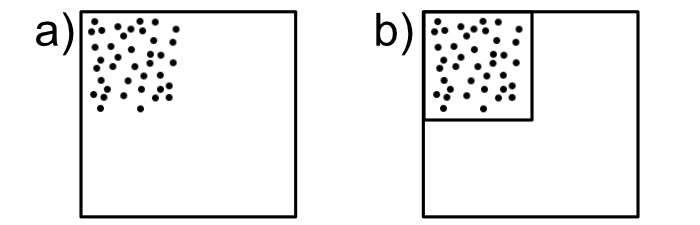
\includegraphics[width=12cm]{Figure1} \caption{Gas enclosed in part of a container - two non-equivalent cases.}
\label{Fig1} 
\end{figure}

The means of practical use of still non-coarse-grained entropy in closed systems subject to an adiabatic change was explained with the use of MaxEnt approach by Jaynes \cite{Jaynes:1965gg}. If we knew that on the beginning, at time $t_0$ the system is in \textit{complete} thermodynamic equilibrium having entropy $S$, then we know that at the later time; after the external adiabatic influence ceased the new "test" or experimental distribution function will have entropy $S_e \geq S$. By saying that we demand \textit{complete} thermodynamic equilibrium at the beginning, we say that the \textit{systems history} has to be followed by the experimenter in order to become confident of the obtained equilibrium, as some otherwise unexplainable exceptions exist, such as the Hahn experiment \cite{Hahn:1950zz}.

It is perhaps worth underlying, that the increase of entropy is linked to our knowledge about the system, rather than anything it is doing internally. This should not come up as particularly surprising as our division between work and heat is somewhat arbitrary. In fact, as just seen, Jaynes advocated an interpretation of entropy as a measure of reproducibility, rather than disorder \cite{Jaynes:1957zz}.
Furthermore, even the exact parameters of entropy depend on the situation, so does their number. One can increase their number arbitrarily moving toward classical deterministic description where the notion of entropy collapses\footnote{This is not the case for von Neumann entropy.}.

\subsection{von Neumann entropy during measurement process}

Although this work is meant to stay within the classical limit, it might be worth while to clear out the notion of entropy in quantum context.

The von Neumann entropy is defined as 
\begin{equation}
  S_{vN}= -\Tr(\hat{\rho} \log{\hat{\rho}}).
\end{equation}
For which the general form of the density matrix operator is
\begin{equation}
	\hat{\rho}=\sum_k p_k \ket{\psi_k}\bra{\psi_k} .
\end{equation}
For the case of pure state $\ket{\psi}$ the density matrix is simply
\begin{equation}
  \hat{\rho} = \ket{\psi}\bra{\psi},
\end{equation}
and it is easy to verify that the entropy of a pure state is equal to zero. The entropy of mixed state is always greater than zero.
If the system is in a pure state, it will continue to be in a pure state as long as it stays isolated. For a mixed state, the degree of non-purity measured by the entropy will stay constant as long as it is isolated. This follows from the fact that the time evolution is unitary and the eigenvalues of the density operator do not change in time under such conditions.

An interesting question one might ask (and not really discussed in textbooks) is how the entropy changes after a measurement of a particle in many-body system which, initially, was in pure state.

Without loss of generality, let's consider an isolated system of two identical particles described solely by their momentum states.
In the scenario of two particles of identical momentum we can write the initial pure state as 
\begin{equation}
  \ket{2,0,0,...}
\end{equation}
which has, of course, zero entropy. Now we would like to perform a measurement on that state. 
In the second quantization formalism the measurement of a particle is realized by the field operator $ \hat{\Psi}(x) =\sum_k \phi_k(x)\hat{a}_n$, which annihilates a single particle at position $x$.
Therefore after the measurement of particle at some position $x$, one particle is "virtually" removed from the system under consideration, but the system stays in pure state
\begin{equation}
  \hat{\Psi}(x)\ket{2,0,0,...}=\phi_1(x)\ket{1,0,0,...},
\end{equation}
with zero entropy. It is important to notice though, that a particle is lost from our considerations and therefore the entropies before and after the measurement describe two different systems. Of course, in reality the particle doesn't disappear. After determination of its position by experiment ($\Delta x \to 0$), the uncertainty of its momentum approaches infinity ($\Delta p \to \infty$), which means that we can reconstruct the real state using a linear combination of states with \textit{any} value of momentum:

\begin{equation}
  c_1\ \ket{2,,0,...}+c_2\ \ket{1,1,0,...}+  c_3\ \ket{1,0,1,...}+...
\end{equation}
where the  squared modulus of the coefficients has to sum up to one ($ \sum_i \left| c_i \right|^2 = 1 $).

Now depending on the precision of the measurement we can recalculate our entropy, now getting a value greater than zero. If we would perform the same analysis for a pure state of two particles in different states i.e. $\ket{1,1,0,...}$ then we would obtain an increase of entropy even without accounting for the lost particle.
%TODO Correct also for correlated systems?
This crude example gives a clear illustration of the fact that after \textbf{any} measurement the von Neumann entropy has to increase and that its change is ultimately related to lost information about the system in the act of the measurement.

There's another interesting feature of quantum entropy, namely inequalities that it fullfills.
If we bipartite the system into subsystems $A$ and $B$ each containing its own set of commuting observables, then in order to calculate the entropy $S_A$ of a subsystem $A$ we need to calculate the entropy with respect to density matrix traced over the other subsystem, namely
\begin{equation}
  \hat{\rho}^A = \Tr_B \hat{\rho},
\end{equation}
then in general the following identities are satisfied

\begin{equation}
\begin{aligned}
	S(\rho) &\leq S_A + S_B	\\
	S(\rho) &\geq \left| S_A - S_B \right|.
\end{aligned}
\end{equation}

The interpretation of the first inequality is that the full information about the states of the subsystems $A$ and $B$ will in general not be sufficient to give full information about the state of the total system $A+B$. Or in other words, when there are correlations between the two subsystems, these are not seen in the description of $A$ and $B$ separately. 

\section{Near-equilibrium thermodynamics}
\label{NearEquilibrium}
\subsection{Local equilibrium and entropy production}

The term \textit{local equilibrium} describes the situation in which the thermodynamic quantities of the system such as density, temperature, pressure, etc. can vary spatially and with time, but in each volume element the thermodynamic relations between the values which apply locally are obeyed. 
Such conditions are possible through the assumption of efficient dissipation of effects imposed by gradients and chemical affinities through molecular collisions. We therefore expect that this to hold for fluids, moderately dense gases and many solids.
Under this assumptions, extension of equilibrium thermodynamics is possible \cite{Anonymous:NJxQY1gt}.

An approach pioneered by Onsager, describing entropy in case of open systems, is an extension of Clausius entropy for isolated systems. It states that the variation of system's entropy $dS$ is the sum of two contributions: 
\begin{equation}
\label{OpenSystemEntropy}
  	dS=dS_i+dS_e,
\end{equation}
the entropy produced within the system $dS_i$ (for example by change of microscopic configuration) and the entropy transferred into (or out of) the system through its boundaries $dS_e$.

The Second Law then states that internal entropy production $dS_i$ must be zero for reversible (equilibrium) transformations and positive for non-equilibrium transformations of the system \cite{DeGroot:2013ue}:
\begin{equation}
  dS_i \geq 0,
\end{equation}
or per unit time:
\begin{equation}
  	\frac{dS_i}{dt}=\int \sigma dV \geq 0
\end{equation}
where $\sigma$ is the entropy production source per unit volume and $dV$ denotes infinitesimal volume element.

The entropy supplied, $dS_e$, on the other hand may be positive, zero or negative, depending on the interaction of the system with its surroundings and may be written in terms of entropy flows through the boundaries of the system:
\begin{equation}
  	\frac{dS_e}{dt}=\int J d\Omega,
\end{equation}
where $J$ denotes the flux and $d\Omega$ the infinitesimal element of the boundary of the system. For a closed system we have the Clausius relation in terms of exchanged heat:
\begin{equation}
  dS_e=\frac{dQ}{T}.
\end{equation}


The standard formalism of linear irreversible dynamics develops then a more explicit expression for entropy production per unit time, assuming that even outside equilibrium (but near) entropy depends only on the same variables as at equilibrium, expanding it as follows: 

\begin{equation}
  \sigma(x,t) = \sum_i J_i(x,t) X_i(x,t) \geq 0.
\end{equation}


The sources of entropy production from the point of view of coarse-grained Gibbs entropy have been intensely studied in non-equilibrium systems. A notable result \cite{Gilbert:1999ff, Goldstein:1998ip} states that entropy production itself is independent of the level of coarse-graining applied to Gibbs entropy.

There exist however some conceptual problems with the assumption of non-negative entropy sources.
For example in an electric circuit close to equilibrium, entropy production is equal to the product of the electric current times the voltage divided by the ambient temperature. If the circuit has a complex impedance, there will necessarily be a phase lag between the applied voltage and the current. Therefore there will exist an interval in which entropy production will be negative.
This fact was noted by Landauer in his analysis \cite{Landauer:pJ4RYJRG} of Glansdorff's and Prigogine's book \cite{Anonymous:NJxQY1gt}. The modern far from equilibrium approach, involving fluctuation theorems and \textit{dissipation function} solves this problem \cite{Evans:2241458}.

\subsection{Linear response, regression and fluctuations}

A very common approximation made in the treatment of near-equilibrium thermodynamics is the assumption of linear response. If an adiabatically insulated system is perturbed out of equilibrium (but still very near to it) by some time dependent force $f(t)$, then the response of mean zero observable $\delta X= X-\langle X \rangle_{eq}$  should satisfy the linearity property

\begin{equation}
\label{LiearityProperty}
  \delta X(\lambda f(t),t) = \lambda \delta X(f(t),t)
\end{equation}

Linear response of a system driven from equilibrium can be described in terms of the \textit{time correlation (autocorrelation) function} of the observable $X$ (from now on we will assume that $X$ is mean zero observable, that is $X=\delta X$):
 
\begin{equation}
  C(t)=\langle X(t)X(0) \rangle = \frac{\Tr{X(t)X(0)\rho_{eq}}}{\Tr{\rho_{eq}}}.
\end{equation}
% Change Tr to integrals?
where $\rho_{eq}$ is the equilibrium density function.

With the use of correlation functions, we now study the effect of relaxation towards equilibrium, assuming that the external influence ceased at time $t=0$.
Then a general property of such auto-correlation function for times $t\geq 0$ is called \textit{regression} and follows directly from the Schwarz inequality and $X^2(t)<X^2(0)$ - the assumption of fading disturbance:
\begin{equation}
 | C(t) | \leq C(0).
\end{equation}
In fact in the long time limit we expect to obtain the equilibrium values of observables and
\begin{equation}
  \lim_{t \to \infty} C(t)=0.
\end{equation}

Some further properties useful for further discussion can also be noted.
On the microscopic level of enumerated, time dependent observables $X_i$, the equations of motion are time reversible and time translation invariant \cite{Anonymous:vN0-ttAB}, thus leading to\footnote{Some of the variables $X_i$ can in fact be odd under time reversal, thus for those $\langle X_i(t+\tau) X_j(t) \rangle = \langle -X_i(t) X_j(t+\tau) \rangle$.}:
\begin{equation}
  \langle X_i(t+\tau) X_j(t) \rangle =   \langle X_i(t-\tau) X_j(t) \rangle =  \langle X_i(t) X_j(t+\tau) \rangle.
\end{equation}
Dividing by $\tau$ and going with it to the limit $\tau \to 0$ we obtain: 

\begin{equation}
\label{CorrelationTimeDerivative}
  \langle \dot{X}_i(t) X_j(t) \rangle = \langle X_i(t) \dot{X}_j(t) \rangle.
\end{equation}

Now, one might perform an analysis from the macroscopic view.
Assume that some system is described by a set of macroscopic variables $\{\bar{X}_i\}$ for $i=1,...,N$ of zero mean $E(\bar{X}_i)=0$, such that a non-zero value of $\bar{X}_i$ corresponds to an average deviation from the equilibrium value due to an applied external force $f$. Again we'll assume the case in which the force ceases to exist for $t>0$. From experience one then postulates a set of phenomenological coupled equations bringing the system back to equilibrium state: 
\begin{equation}
\label{LinearResponseEq}
  \dot{\bar{X}}_i=-\sum_j \lambda_{ij} \bar{X}_j.
\end{equation}
Such coupling between macroscopic variables is the source of many old relations, such as thermoelectric Peltier and Seeback effects. The probability of such deviations is then proportional to the phase volume given by exponential of entropy change (see \ref{Gibbs entropy}):

\begin{equation}
  P \propto \exp(\frac{S(\bar{X}_1,...,\bar{X}_N)-S_0}{k_B}),
\end{equation}

where $S_0$ is the equilibrium value of entropy. Since we consider near-equilibrium, the linear term in the expansion disappears and we're left with
\begin{equation}
  S-S_0 = - \sum_{ij} S_{ij}\bar{X}_i \bar{X}_j,
\end{equation}
where $S_{ij}= -\frac{1}{2}\frac{\partial^2{S}}{\partial{\bar{X}_i}\partial{\bar{X}_j}}$ is a positive definite, symmetric matrix. %Check on this later

One then defines so-called \textbf{generalized thermodynamic forces} as
\begin{equation}
  F_i= -\frac{\partial{S}}{\partial{\bar{X}_i}}= \sum_j S_{ij}\bar{X}_j.
\end{equation}
From which, by matrix inversion one can obtain again the macroscopic variables $\bar{X}_i$:
\begin{equation}
  \bar{X}_j = \sum_i (S^{-1})_{ji} F_i.
\end{equation}
Inserting those back to equation (\ref{LinearResponseEq}) one gets
\begin{equation}
\label{FluxesOnMacroscopic}
  \dot{\bar{X}}_i=-\sum_j \lambda_{ij} \sum_k (S^{-1})_{jk} F_k = \sum_k \gamma_{ik} F_k.
\end{equation}

\subsection{Onsager relations and hypothesis}
\label{OnsagerRelationsSection}

Lars Onsager \cite{Onsager:zgWBDrcO} shown that $\gamma_{ik}$ from the previous paragraph is in fact symmetric. We can now repeat his derivation just that by combining the equation (\ref{CorrelationTimeDerivative}) with equation (\ref{FluxesOnMacroscopic}), thus obtaining Onsager relations:

\begin{equation}
\label{OnsagerRelations}
  \gamma_{ij}=\gamma_{ji}.
\end{equation}

In general the relaxation of small macroscopic non-equilibrium disturbances need not to be related to the regression of microscopic fluctuations in the corresponding equilibrium system. 
However, Onsager conjectured that in the linear approximation they should be equal. To see why this is the case we give a heuristic argument for mechanical forces.
If we assume that the external force $f$ couples to the observable $X$ then the Hamiltonian will exhibit an additional\footnote{This comes from small displacements approximation and $f=-\frac{\partial}{\partial{X}} H$.} term $H'=-f X$.
Let's now consider the expression for $\bar{X}$ for time $t < 0$:
%TODO: Justify the approximation a bit better
\begin{equation}
  \bar{X}(0)=\frac{\Tr\{ X(0) e^{-\beta (H-f X)} \}}{\Tr\{ e^{-\beta (H-f X)} \}} \approx \beta f \langle X(0)X(0) \rangle= \beta f C(0),
\end{equation}
where in approximation each exponential was Taylor expanded to first order.
For time $t>0$:

\begin{equation}
  \bar{X}(t)=\frac{\langle X(t) e^{-\beta (H-f X)} \rangle}{\langle e^{-\beta (H-f X)} \rangle} \approx \beta f \langle X(t)X(0) \rangle= \beta f C(t).
\end{equation}
Onsager hypothesis can now be seen as simply:
\begin{equation}
  \frac{\bar{X}(t)}{\bar{X}(0)}=\frac{C(t)}{C(0)}.
\end{equation}
As a practical note on application of Onsager relations, we quote Charles Kittel \cite{Kittel:817295}:
\begin{displayquote}
"It is rarely a trivial problem to find the correct choice of (generalized) forces and fluxes applicable to the Onsager relation."
\end{displayquote}

\subsection{Green-Kubo relations}

The Green-Kubo formulae relate the macroscopic, linear transport coefficients of a system to its microscopic equilibrium fluctuations.
A foretaste of the Green-Kubo formalism was already given in the previous section where we considered a small perturbation term $H'=-f X$ to the Hamiltonian $H$. However to keep the presentation simple we will now turn our attention to isothermal case and static force $f$.
The term for small macroscopic deviations of $Y$ due to field $f$ is given by
\begin{equation}
\bar{Y}=\frac{\Tr\{ Y e^{-\beta (H-f X)} \}}{\Tr\{ e^{-\beta (H-f X)} \}} = \Tr\{ Y e^{-\beta (H - F -f X )} \}
\end{equation}
where $F$ denotes the free energy coming from the partition function. The linear response approximation defines the static isothermal ($T$) susceptibility $\chi_{BA}^T$ by\footnote{Note, that here again $Y$ is assumed to have mean zero.}:
\begin{equation}
  \bar{Y} =\chi_{YX}^T f.
\end{equation}
With the use of the following identity \cite{Kubo:1957cl}:
\begin{equation}
  e^{\beta (a+b) }=e^{\beta a} (1+\int_0^{\beta} d\lambda\ e^{-\lambda a} b e^{\lambda (a+b)}),
\end{equation}
with $a=H-F$ and $b=-f X$. One can notice that the integral part corresponds to the change in density function under which the ensemble average takes part, thus
\begin{equation}
\begin{aligned}
  \bar{Y} &= \int_0^{\beta} d\lambda\ \Tr\{ Y e^{-\lambda (H - F)} X e^{\lambda (H-F-f X)} \} f \approx  \int_0^{\beta} d\lambda\ \Tr\{ Y e^{-\lambda (H - F)} X e^{\lambda (H-F)} \} f \\
  &= \langle Y X \rangle f,
\end{aligned}
\end{equation}
where by approximating $f X$ to be small we obtained a special case of Green-Kubo relations defining the cross term susceptibility between observables $X$ and $Y$ in terms of correlation functions in the static force, isothermal conditions:

\begin{equation}
  \chi_{YX}^T = \langle Y X \rangle.
\end{equation}

As a note, let's mention a famous objection to the Kubo relations poised by van Kampen. The argument of van Kampen concerned the plausibility of taking the linear terms first and then the ensemble average (in general one should do the opposite). An answer to this objection is that the microscopic trajectories of particles affected by the perturbing fields experience a large number of collisions in exceedingly small times ($\approx 10^{-9}s$ for low density gases) which makes the approximation possible \cite{Dorfman:ozm67-zD}.
\subsection{Steady states and the definition of temperature}

The steady state is loosely defined as an emergent state of a system sustained by some constant\footnote{Constant in the sense of some finite-time $\tau$ average.} driving force $F_e$ or constant fluxes vector $\bm{f}$, for which the values of various observables denoted as $A_i$ converge and stabilize after a sufficiently long time, i.e.
\begin{equation}
\begin{aligned}
  \lim_{t \to \infty} \langle A_i(t) \rangle_0 = const,\\
  \frac{1}{\tau} \int_0^{\tau} F_e(t) dt =const,
\end{aligned}
\end{equation}
where "const", in the first case, denotes some different (for each $i$) constant values and the ensemble average here is taken with respect to initial probability distribution function.

In some cases, one can impose a condition of vanishing expectation value of $\partial \rho / \partial t$ over the probability density function $p(\rho)$ and non-vanishing expectation value of fluxes vector $\bm{f}$ over the probability density function $p(\bm{f})$ \cite{Dewar:2014ek}, i.e.
\begin{equation}
\begin{aligned}
\label{SteadyStates}
  \langle \frac{\partial \rho}{\partial t} \rangle_{p(\bm{\rho})} &= 0 \\
  \langle \bm{f} \rangle_{p(\bm{f})} &\neq 0.
\end{aligned}
\end{equation}
The first definition (constancy of the density function) cannot however strictly hold. Indeed, in cases far from equilibrium considered in section \ref{DissipationTheoremSection} it is shown to be false. This case is used as approximation in the MaxEP approach of section \ref{MaxEPInferenceSection}.

When discussing steady states one often uses Clausius entropy to describe entropy changes related to heat transfer, however the temperature used in its definition is not always well defined. In cases of near-equilibrium that one may call local equilibrium, the definition of temperature differences are "smooth" enough, i.e. locally there is a reasonable definition of temperature and the temperature gradient determines the heat flux. 
In the opposite case, it is the molecular kinetics which determines the energy transfer. In most cases under consideration it happens much faster and is considered a transient state after which local equilibrium gets established.

On the other hand, in far from equilibrium conditions there might be several definitions of temperature. One of the solutions provided by Evans et al. \cite{Evans:2241458} is to define temperature of non-equilibrium state by the temperature of the underlying equilibrium state to which the system would otherwise relax. This definition gives consistent results.

\subsection{MinEP principle}

The most well known contribution of Ilya Prigogine to statistical physics, often called the Minimum Entropy Production (MinEP) principle, sprouts from the analysis of second order excess entropy around a steady state $ (\delta^2 S)_{ss} $. 

If we perturb the system around its equilibrium state we obtain:
\begin{equation}
  S=S_0 + \delta S + \frac{1}{2}\delta^2 S,
\end{equation}
the linear term, $\delta S$, vanishes near equilibrium, the latter is a quantity later used as a Lyapunov function and has certain benefits over other (not necessarily all) Lyapunov functions one could define. 
It's macroscopic meaning is conserved independently of microscopic details of the system under consideration and is also independent of the nature of particular (possibly inhomogeneous) fluctuations.

The MinEP principle generated considerable excitement initially, for it enabled prediction of the long-time behaviour of the system by optimizing one collective thermodynamic property of the end state. Its validity, however, is restricted to near-equilibrium steady-states. It is not a general selection principle, neither does it imply nor is it a consequence of another principle that could lead to the emergence of complexity\footnote{In contrast to MaxEP described in section \ref{UnifyingPrinciple}.}. 
Only near-equilibrium the quantity $ (\delta^2 S)_{ss} $ generates probability of fluctuations, as Prigogine himself, later insisted in response to criticism \cite{Nicolis:1979cv}.

This is in contrast to the term "dissipative structures" also coined by Prigogine, who initially proposed that many properties of dissipative structures, referring to biological organization, could be explained by a general thermodynamic tendency to reduce the rate of entropy production. In Prigogine's view the fluctuations are the trigger for the instabilities (or rather bifurcations in the equations of motion), which in turn give rise to spacetime dissipative structures. 
An often given example of instabilities leading to formation of structures are the Rayleigh-Bénard convection cells, which simplified non-equilibrium (not near-equilibrium nor MinEP) treatment is described in the next section.


\section{Thermodynamic lowering of entropy in non-equilibrium conditions}
\label{simple-model}

The Second Law of course holds for isolated systems as a whole and one can therefore imagine (on the basis of additivity of entropy) that out of equilibrium some subsystems may maintain lower entropy.

Let's therefore consider a simple model consisting of three elements: the cooler $C$, the heater $H$ and a system under consideration $S$, staying out of equilibrium.
We assume, that the temperatures of the cooler and the heater stay constant, and that heat $Q_H$ flows into the system $S$ and heat $Q_C$ flows out. The situation is illustrated by the figure \ref{Fig2}.
\begin{figure}[ht!]
\centering 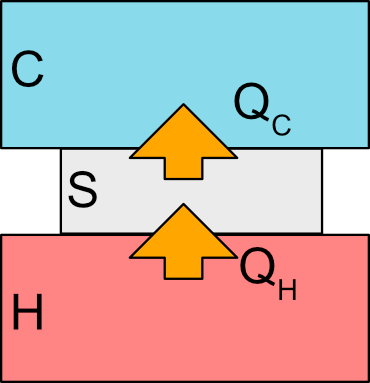
\includegraphics[width=6cm]{system} \caption{System (S) under the conditions of continuous heat transfer.}
\label{Fig2} 
\end{figure}
Treating the heater and the cooler as the environment, we can think of our system $S$ as an open (but without particle transfer).
Further on we will analyze the system $S$ from the perspective of internal $(i)$ entropy production and external $(e)$ entropy flux, flowing \emph{to} the system $S$. 
The change in entropy, as in equation (\ref{OpenSystemEntropy}), will be the sum of those two contributions:
\begin{equation}
dS_S=dS_i+dS_e.
\label{entrosum}
\end{equation}
In the current analysis let's consider a steady state situation in which the same amount of heat flows in as flows out, that is $dQ_C=-dQ_H$. Using this relation we get the following term for the change of entropy:
\begin{equation}
dS_e=\frac{dQ_H}{T_H}+\frac{dQ_C}{T_C}=dQ_H\left(\frac{1}{T_H}-\frac{1}{T_C}\right)
=dQ_H\left(\frac{T_C-T_H}{T_HT_C}\right)<0.
\label{dSe1}
\end{equation}
From which it follows, that the heat flow takes the entropy out of our system.
For the purpose of further discussion we introduce the concept of rate of entropy change connected with the heat flow:
\begin{equation}
j_e \equiv  \frac{dS_e}{dt}. 
\end{equation}
In the considered scenerio, the $j_e$ is held constant (steady state) and we suspect a continuous fall in system's entropy. Yet, moving away from the equilibrium state we suspect, that the a balancing role will be played by $dS_i$ moving the system back to equilibrium state. Similarly, as before we define the rate of internal entropy production:
\begin{equation}
j_i \equiv \frac{dS_i}{dt}.   
\end{equation} 
When $T_H=T_C$, i.e. the system is in equilibrium with constant entropy $S_{EQ}$, therefore it follows that $j_i=0$.
We assume that the rate of internal entropy production $j_i$ should be a function  of system's entropy $S_S$, i.e. $j_i = j_i(S_S)$ with the boundary condition $j_i(S_S=S_{EQ})=0$. Around the equilibrium state $S_S=S_{EQ}$, we can Taylor expand the function $j_i(S_S)$ to its linear term
\begin{equation}
j_i(S_S)=j_i\left(S_{EQ}\right)+\left(S_S-S_{EQ}\right)C_1+\mathcal{O}\left(S_S^2\right),
\end{equation} 
fulfilling $j_i\left(S_{EQ}\right)=0$. The dimensional and stability analysis tells us that $C_1$ has the dimension of inverse time and in the case of 
$j_e=0$ should simply be equal to $S_{EQ}$, therefore we set $C_1 = -\frac{1}{\tau}$, where $\tau$ is a positive defined relaxation constant. Using the equation (\ref{entrosum}) we get
\begin{equation}
\label{stab}
\frac{dS_S}{dt}=j_i\left(S_S\right)=\left(S_S-S_{EQ}\right)C_1.
\end{equation} 
The solution of the differential equation (\ref{stab}) is given by:
\begin{equation}
S_S(t) =S_{EQ}+(S_0-S_{EQ})e^{-t/\tau}, 
\end{equation}
where the initial condition was set $S_S(0)=S_0$. Now we include the term $j_e$ into our considerations.
In this case the equation (\ref{entrosum}) results in the following differential equation:
\begin{equation}
\frac{dS_S}{dt}=j_e + j_i\left(S_S\right)=j_e +\frac{S_{EQ}-S_S}{\tau}.
\label{dSSdt}
\end{equation} 
Given the boundary condition $S_S(0) =S_{EQ}$ its solution is given by:
\begin{equation}
S_S(t)=S_{EQ}+j_e\tau \left(1-e^{-t/\tau }\right),
\end{equation} 
where $j_e$ is a negative constant. The graph of this function is presented on figure \ref{Fig3}. 
One can see that in the limit $t\rightarrow \infty$ the entropy of the system falls to its minimal value:
\begin{equation}
S_{min}=S(t\rightarrow \infty) =S_{EQ}+j_e \tau < S_{EQ}.
\end{equation}

\begin{figure}[ht!]
\centering 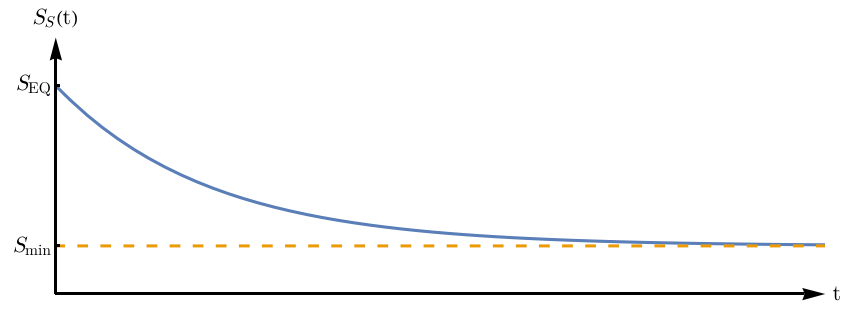
\includegraphics[width=12cm]{wykres3} 
\caption{Lowering of entropy induced by heat flow as a function of time.}
\label{Fig3} 
\end{figure}

This is of course consistent with the second law of thermodynamics as we are describing an open system.
It is easy to notice that the total entropy change is equal to $dS=dS_i \geq 0$ (for simplicity it was assumed that the heater and cooler don't act as producers of entropy).
We see that if the relaxation constant $\tau = 0$, then the system would stay in equilibrium the whole time, of course, $\tau > 0$ for most materials (if not all). The most important part due to which this low entropy state was obtained is of course the entropy out-flow $j_e$, without which the non-equilibrium condition allowing for growth of complexity would not form.

\section{General measure of irreversibility and the Second Law}
\label{IrreversibilityMeasureSection}
In the following section we propose a general measure of irreversibility which is closely related to the presented later fluctuation theorems. It is derived using nothing else than simple probability calculus and the hypothesis of equal a priori probabilities.
The result that we will obtain at the end of this section is an exact form of the entropy produced in terms of microscopic transition rates given by random matrices. The character of the obtained distributions will depend only on the ratio of the number of the initial macroscopic states and the number of the final macroscopic states.

Let's consider a generic statistical mechanical system at two times, at initial time $t_0$ and at final time $t_1$, each described by a complete set of possible macrostates $\{A_i\}$ for $ i=1,...,N_A $ and $\{B_j\}$ for $ j=1,...,N_B $  respectively. Each initial macrostate consists of some number of corresponding microstates denoted by $M_i$, and similarly, each final macrostate consists of some number of final microstates denoted by $N_j$. The deterministic, microscopic equations of motion then evolve a certain number of the microstates $K_{ij}$ from an initial macrostate $A_i$ to some final macrostate $B_j$, as illustrated on figure \ref{Fig4}.
\begin{figure}[ht!]
\centering 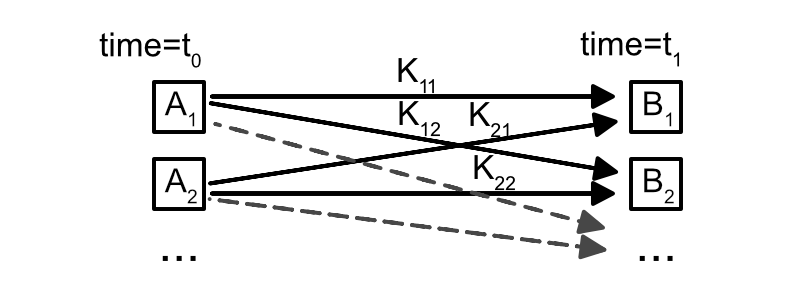
\includegraphics[width=15cm]{figure4} 
\caption{Transitions between macrostates ${A_i}$ and macrostate ${B_i}$ dictated by the 'transition' matrix $K_{ij}$.}
\label{Fig4} 
\end{figure}
The probability of the forward transition $P(B_j|A_i)$ is then equal to
\begin{equation}
\label{ForwardProb}
  P(B_j|A_i)= \frac{K_{ij}}{M_i}.
\end{equation}
Now for the time reversed case, that is to obtain $P(A_i|B_j)$, we use the \textit{extended Bayes theorem}
\begin{equation}
  P(A_i|B_j)=\frac{P(B_j|A_i)P(A_i)}{\sum_k P(B_j|A_k)P(A_k)},
\end{equation}
remarking that $A_i$ is our hypothesis and $B_j$ is our evidence. Now, since we have no a priori knowledge about the initial macrostates, each of them is equally probable $P(A_i)= 1/N_A$. Using this and equation (\ref{ForwardProb}) we obtain the following expression for the post-diction:
\begin{equation}
\begin{aligned}
  P(A_i|B_j) &= \frac{K_{ij}}{M_i} P(A_i) \left( \sum_k \frac{K_{kj}}{M_k}P(A_k) \right)^{-1}\\
  &= \frac{K_{ij}}{M_i} \left( \sum_{k} \frac{K_{kj}}{\sum_m K_{km}} \right)^{-1},
\end{aligned}
\end{equation}
where in the last equation we made use of the fact that $\sum_m K_{km}=M_k $.
It is important to emphasize that the conditional probabilities $P(B_j|A_i)$ and $P(A_i|B_j)$ are entirely different in nature - the first represents a prediction, but the second is a post-diction. There is no symmetry between assumptions and assertions in conditional probability calculus.

Now, comparing the probability of forward macroscopic evolution to backward evolution probability one obtains: 

\begin{equation}
\label{MacrostatesPRatio}
  \frac{P(B_j|A_i)}{P(A_i|B_j)}= e^{\ln{\sum_{k} \frac{K_{kj}}{\sum_m K_{km}}}}.
\end{equation}
%TODO: Show that its positive for all cases!
The interpretation of the term in the exponent, can be done by noticing that there's only one known probabilistic quantity\footnote{Up to a numerical factor of $k_B^{-1}$.} that   grows in accord with the more probable events, namely the standard measure of irreversibility - the change of entropy.
We have thus described the entropy produced by a macroscopic system solely in terms of microscopic transition probabilities between some number of macroscopic states, without any assumptions about the dynamics. 

With the use of random matrices filled with uniformly distributed integers from some interval $[0,Z], Z \in \mathbb{N}$, representing numbers of microscopic states transitioning between initial and final macrostates one can obtain the probability distributions for the possible values of $\Delta S = \ln{\sum_{k} \frac{K_{kj}}{\sum_m K_{km}}} $, entropy produced in the transitions. The obtained distributions suggest that if our knowledge about the system stays in tact (no change in number of macroscopic states), then entropy most likely will not change (yellow graph from figure \ref{Fig5})\footnote{If we were to graph the term $\sum_{k} \frac{K_{kj}}{\sum_m K_{km}}$ alone (without the $\log$) then we would obtain perfectly symmetrical distribution.}.
\begin{figure}[ht!]
\centering 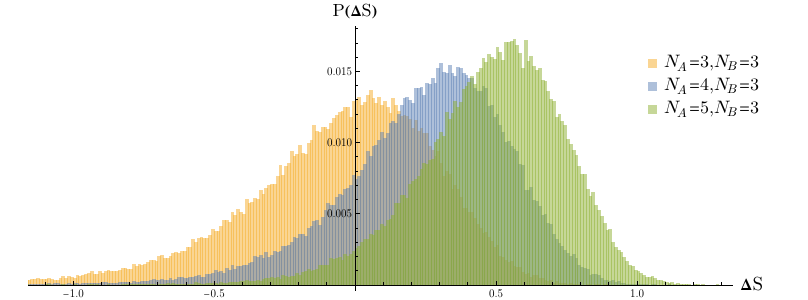
\includegraphics[width=15cm]{Figure5} \caption{Probability distributions of entropy produced in transitions between $N_A$ initial and $N_B$ final macrostates, calculations performed for $N=10^5$ random matrices.}
\label{Fig5} 
\end{figure}
However, if a loss in our knowledge about the system occurs (the number of macroscopic states decreases), then the entropy will most likely increase (blue and yellow graphs from figure \ref{Fig5}). This can be seen most easily on an information theoretical example of a simple logic gate, which irreversibly transforms one of four input states $00,01,10,11$ into one output. With the increasing ratio of initial to final macrostates the probability of spontaneous return due to random heat fluctuations decreases, in accordance to the Second Law.
Hence, our result can be seen as a direct and visual argument against Loschmidt.

A remarkable feature of this results is that the obtained distributions indicate a generalization of the Second Law, quantifying the probability of reverse transitions. This feature is a general characteristics of the so-called fluctuation theorems to which our result most likely belongs.
The exact relation to the known fluctuation theorems will follow in further works, here instead we focus our attention on them in general.

\section{Fluctuation theorems}
\label{FluctuationTheorems}

The fluctuation theorems and their derivatives including Jarzynski equality have been demonstrated for a wide range of systems and in a number of experiments including DNA stretching \cite{Collin:2005fx}, optically trapped colloids \cite{Carberry:2007be}, shearing systems \cite{Evans:1993bl}, pendulums \cite{Ciliberto:2010jg}, molecular motors \cite{Seifert:2005it} and various quantum mechanical systems \cite{Monnai:2005ke}.
%TODO: Extract references from evans_chapter_rev.pdf

Since the development of the first fluctuation theorem of Evans, Cohen and Morriss the conditions of applicability were heavily researched and in the result there exist many approaches for deriving fluctuation theorems. 
Those can be roughly described as deterministic \cite{Evans:2002gg, Evans:2241458} or stochastic \cite{Kurchan:1998, Searles:1999fz}.

In the deterministic framework of Evans, irreversibility finds its origins in non-linear terms which provide the contraction of phase space, this is in contrast to the stochastic descriptions in which irreversibility is given a priori - it can be perceived as merit, for one finds fewer technical difficulties \cite{Crooks:2008ta}. 
In fact, the Gallavotti-Cohen theorem, which is a stationary fluctuation theorem for systems in contact with a deterministic Gaussian thermostat, breaks down in some systems and in most cases when the forcing is very strong.  
Those technical difficulties have their source in ergodicity. The fluctuation relation in the deterministic case holds only if the system has certain ergodic properties \cite{Kurchan:2009ub}. Putting it simply, if the aim of ergodic theory is to understand how randomness arises from deterministic constituents, once stochasticity is added "by hand" the question is artificially bypassed. 

However, the assumption that stochastic processes retains its stochastic character at arbitrary small temporal and spatial scales leads to a conclusion that the rate of production of entropy is infinite at the limit of infinite resolution \cite{Dorfman:ozm67-zD}.

Despite of the acknowledged difficulties, the deterministic approach of Searles and Evans will be described for reasons of generality, aesthetics and also because it distances itself from the notion of entropy.

\subsection{The deterministic approach}


The main objective of this section will be the derivation of the dissipation function and Evans-Searles fluctuation relation (theorem), while introducing the bare minimum amount of necessary concepts. On basis of this results the Crooks fluctuation theorem and Jarzynski equality will then be derived. In the following considerations we will assume that classical mechanics gives an adequate description of the dynamics. We will also assume that quantum and relativistic effects can be safely ignored.

\subsubsection{Thermostated, but time reversible systems}

The construction of thermostated time reversible systems is usually done inserting some time-reversible, but non-Hamiltonian terms into the equations of motion defined as the surroundings. Surroundings in first approximation are assumed to stay far from the system of interest and should not affect the system under consideration.
The work done on a system, should be on average, converted into heat, which is conducted through the system of interest and eventually removed by the non-Hamiltonian terms residing usually, in the remote boundaries.

For Gaussian isokinetic thermostat the mentioned time-reversible term is usually of the form $- S_i \alpha p_i $ where $\alpha$ is determined by the thermostatting condition\footnote{By such construction, the system will relax to an equilibrium state $f_{eq}(\bm{\Gamma})=Z^{-1} e^{-\beta H}\delta(\bm{p}\cdot \bm{S}\cdot \bm{p}-2m K)$ where $K$ denotes the kinetic energy of the system and $Z$ the partition function.}
%\footnote{In the case of Nosé Hoover thermostat, $\alpha$ becomes an extra degree of freedom\cite{Evans:2241458}.}
 and $\textbf{S}$ is a diagonal matrix. The term serves as a mean by which we can add or remove heat from the particles in the reservoir region ($S_i =1$ for reservoir region and $S_i = 0$ outside this region).

In case of isolated hyperbolic systems, interacting with a thermostat the phase space is usually contracted to an attractor and the sum of Lyapunov exponents is less then zero.
This is in contrast with time-reversibility of the thermostated equations of motion. The solution to this apparent paradox is related to the fractal nature of the attractor.
The attractor can be described by a smooth measure in the unstable directions and a fractal measure in the stable directions.
This kind of measures are known as SRB (Sinai-Ruelle-Bowen) measures \cite{Dorfman:ozm67-zD}.

\subsubsection{Time reversible setup}
Let's consider a closed and adiabatic Hamiltonian system of interacting particles which can exchange energy with its environment in the form of work. For example, it might be desirable to change the mean internal energy, $U=\langle H \rangle$ of the system, by externally manipulating some parameter $\lambda(s)$ (in general dependent on time $s$) in the potential energy function. 
For an externally driven adiabatic system, the rate of increase of $H$ must be identically equal to the rate of work $\dot{W}$ done on the system by the environment, thus
\begin{equation}
\label{AdiabaticWork}
  \dot{W}^{ad} = \dot{H}^{ad} = \dot{\lambda} \frac{\partial{H}}{\partial{\lambda}} +\dot{\bm{q}}\frac{\partial{H}}{\partial{\bm{q}}} +\dot{\bm{p}}\frac{\partial{H}}{\partial{\bm{p}}},
\end{equation}
where the superscript \textit{ad} emphasises adiabatic conditions. 

When an external agent (not described by the potential) does work on a system without changing the underlying equilibrium state of mean energy $U$, we refer to that field as a purely \textit{dissipative field}, denoting it generally by vector $\bm{F}_e$.

In the microscopic picture, the systems phase space $\{\bm{q_1},...,\bm{q_N},\bm{p_1},...,\bm{p_N} \} \equiv (\bm{q},\bm{p})\equiv \bm{\Gamma} $ (where $\bm{q_i}, \bm{p_i} $ are denoting position and conjugate momenta of the particle $i$) evolves according to Hamiltonian equations of motion with additional terms connected with the dissipative field $\bm{F}_e$ and the time-reversible thermostat:

\begin{equation}
\begin{aligned}
\label{ThermostattedEq}
  \dot{\bm{q}} &=\frac{\partial H(\bm{\Gamma},s)}{\partial{\bm{p}}}+\bm{C}(\bm{F})\cdot\bm{F}_e(s), \\
  \dot{\bm{p}} &=- \frac{\partial H(\bm{\Gamma},s)}{\partial{\bm{q}}}+\bm{D}(\bm{F})\cdot\bm{F}_e(s) - \alpha(\bm{\Gamma})\bm{S}\cdot\bm{p}.
\end{aligned}
\end{equation}

Note that the thermostatting term ($- \alpha(\bm{\Gamma})\bm{S}\cdot\bm{p}$) was added to our otherwise adiabatic system in an ad-hoc manner and should not influence the  adiabatic work relation of equation (\ref{AdiabaticWork}), which after the addition of the dissipative field $\bm{F}_e$ reduces to:
\begin{equation}
  \dot{W}^{ad}(\bm{\Gamma},s) = \dot{\lambda} \frac{\partial{H(\bm{\Gamma}},s)}{\partial{\lambda}} - V \bm{J}(\bm{\Gamma})\cdot \bm{F}_e(s)
\end{equation}
where $V$ is the volume of the system, and $\bm{J}(\bm{\Gamma})$ is the dissipative flux due to field $\bm{F}_e(\lambda)$, which one (ignoring the thermostat term) can easily obtain:
\begin{equation}
  V \bm{J}(\bm{\Gamma}) = -\Big(\frac{\partial{H}}{\partial{\bm{q}}}\cdot \bm{C}+\frac{\partial{H}}{\partial{\bm{p}}}\cdot \bm{D}\Big).
\end{equation}
Now, using the First Law of Thermodynamics we can include the thermostat into our considerations, concluding that the rate of heat exchange with the thermostat follows from $\dot{Q}=\dot{H}-\dot{W}$ and is therefore given by
\begin{equation}
  \dot{Q}(\bm{\Gamma},s)= -\alpha(\bm{\Gamma})\frac{\partial{H}}{\partial{\bm{p}}}\cdot \bm{S}\cdot \bm{p}.
\end{equation}
The total work done and heat added to the system then depends only on the initial phase space point $\bm{\Gamma}_0$ and time duration $t$. That is, $W(\bm{\Gamma}_0,t)=\int_0^t \dot{W} dt$ and $Q(\bm{\Gamma}_0,t)=-\int_0^t \dot{Q} ds$.

Introducing the basics of thermostats, we now wish to move back to some more general considerations. 
We define a time reversal mapping $M^T$ (written for short as superscript star) to be an operator acting on phase space (the brackets indicate that the operator acts here on the phase exclusively): 
\begin{equation}
  \bm{\Gamma}^*=M^T[\bm{\Gamma}] \equiv (\bm{q},-\bm{p})
\end{equation}
and a p-Liouvillean operator $iL$ defined by the solution of differential equation 
\begin{equation}
 \dot{\bm{\Gamma}} \equiv iL(\bm{\Gamma})\bm{\Gamma},
\end{equation}
which is given by
\begin{equation}
  \bm{\Gamma}_t = S^t \bm{\Gamma} \equiv \exp[iL(\bm{\Gamma})t]\bm{\Gamma}.
\end{equation}
where the $\bm{\Gamma}_t$ denotes phase evolved to time $t$ and the $ exp[iL(\bm{\Gamma})t] $ is known as the p-propagator or the phase space propagator.
A property useful in later part of this work is:

\begin{equation}
\label{PhaseTimeDer}
  \frac{d}{dt}(S^t \bm{\Gamma})=iL(\bm{\Gamma})\exp[iL(\bm{\Gamma})t]\bm{\Gamma}=S^t \dot{\bm{\Gamma}}.
\end{equation}
%TODO: It doesn't seem perfectly ok...
%left out how M^T acts on iL (page 18)
%\equiv  \dot{\bm{\Gamma}}\cdot \frac{\patial}{\partial{\bm{\Gamma}}}
The time reversal dynamics satisfies an easy to check equation:
\begin{equation}
  M^T S^t M^T S^t\ \bm{\Gamma} = \bm{\Gamma},
\end{equation}
where the action of operators $M^T$ and $S^t$ is evaluated from the right side to the left side. 

The introduced equations indicate to an the existence of time reversed trajectories (anti-trajectories), i.e. if we generate a trajectory starting at $\bm{\Gamma}_0$ and terminating at $\bm{\Gamma}_t$, then under the same dynamics, we start at $\bm{\Gamma}_t^*$ and arrive back to $\bm{\Gamma}_0^*$.
In most cases presented here though, we will be interested in \textit{bundles} of trajectories $d\bm{\Gamma}$ and \textit{bundles} of anti-trajectories $d\bm{\Gamma}^*$ passing through a volume element centered around the point $\bm{\Gamma}$.

We now proceed to introduce a handful of important concepts.

\paragraph{Phase space distribution function:}

The phase space distribution function $f(\bm{\Gamma};t)$ gives the probability per unit phase space volume of finding phase members near the phase vector $\bm{\Gamma}$ at time $t$.

\paragraph{Probabilities of phase space trajectories: }
The probability $p(d V_{\bm{\Gamma}_t},t)$, that a phase $\bm{\Gamma}_t$, will be observed within an infinitesimal phase space volume of size $d V_{\bm{\Gamma}_t}$ about $\bm{\Gamma}_t$ at time $t$, is given by,

\begin{equation}
  p(d V_{\bm{\Gamma}_t},t) = f(\bm{\Gamma}_t;t)d V_{\bm{\Gamma}_t}.
\end{equation}


\paragraph{Ensemble averages:}

Value of any phase function $A(\bm{\Gamma})$ can be obtained with the use of ensemble averages by taking $N_{\bm{\Gamma}} $ time evolved initial phases $\bm{\Gamma}$ consistent with macroscopic constraints
\begin{equation}
  \langle A(t) \rangle = \lim_{N_{\bm{\Gamma}}
 \to \infty} \sum_{j=1}^{N_{\bm{\Gamma}}} A(S^t \bm{\Gamma}_j)/N_{\bm{\Gamma}},
\end{equation}
or in the continuous limit by specifying the initial phase space probability density $f(\bm{\Gamma};0)$ or time-dependent evolution of this density $f(\bm{\Gamma};t)$:

\begin{equation}
  \langle A(t) \rangle = \int d\bm{\Gamma} A(\bm{\Gamma}) f(\bm{\Gamma};t) = \int d\bm{\Gamma} A(S^t\bm{\Gamma})f(\bm{\Gamma};0).
\end{equation}
This equation can be seen as an application of equivalence of Heisenberg and Schrödinger representations - either the observable or the state is evolved.
Time stationarity of an ensemble average is then defined simply by
\begin{equation}
\label{StationaryStateDef}
    \langle A(t) \rangle =   \langle A(t+\Delta) \rangle,
\end{equation}
for any time $\Delta > 0$.

%TODO: More on ensemble averages can be found on page 35

\paragraph{Ergodicity:}
Stationary system is said to be physically ergodic if the time average of the phase function representing a physical observable, along a trajectory that starts \textit{almost anywhere}\cite{Evans:2241458} in the ostensible phase space, is equal to the ensemble average taken over an ensemble of systems consistent with the small number of macroscopic constraints on the system:

\begin{equation}
    \lim_{t \to \infty} \langle A(t) \rangle = \lim_{t \to \infty} \frac{1}{t} \int_0^t ds\ A(S^s \bm{\Gamma}).
\end{equation}
%TODO: Page 22, another definition on page 74

One may also talk about, so-called \textit{ergodic consistency condition} in many context, the reason for this requirement stems from the requirement of existence of distributions sitting in the denominator of various theorems for example in the definition of (later introduced) dissipation function.

\subsubsection{Phase Continuity equation}

%To model a three-dimensional system of $N$ interacting particles, we assume that the microstates were initially distributed according to a given normalized probability distribution function $f(\bm{\Gamma};0)$. As mentioned before we separate our system of $N$ particles into system and surroundings, where the surroundings are assumed to be composed of $N_{th}$ particles. 

%TODO: Construction of the termostat left for later, start at page 24

The motion of the phase space distribution function is governed by a Lagrangian form of the phase continuity equation (also known as \textit{streaming}):
\begin{equation}
\label{LagrangianLiouville}
  \frac{df(\bm{\Gamma};t)}{dt}=-f(\bm{\Gamma};t)\frac{\partial}{\partial \bm{\Gamma}} \cdot \dot{\bm{\Gamma}}(\bm{\Gamma}) = -f(\bm{\Gamma};t)\Lambda(\bm{\Gamma}).
\end{equation}
This equation follows directly from a well known form of Liouville equation
\begin{equation}
    \frac{\partial f(\bm{\Gamma};t) }{\partial t}
    = -\frac{\partial}{\partial \bm{\Gamma}} \cdot [\dot{\bm{\Gamma}}(\bm{\Gamma}) f(\bm{\Gamma};t)]
     = -(\frac{\partial}{\partial \bm{\Gamma}} \cdot \dot{\bm{\Gamma}} + \dot{\bm{\Gamma}} \cdot \frac{\partial}{\partial \bm{\Gamma}}) f(\bm{\Gamma};t),
\end{equation}
where by moving the last term to the left side we get back equation (\ref{LagrangianLiouville}).

%\noindent\makebox[\linewidth]{\rule{\textwidth}{1pt}} 
%\paragraph{}

We say that a system fulfills the \textit{adiabatic incompressibility of phase space} ($AI\bm{\Gamma}$) if in the \textbf{absence} of the thermostatting terms the equations of motion preserve the phase space volume, that is
\begin{equation}
  \Lambda \equiv (\partial / \partial\bm{\Gamma}) \cdot \dot{\bm{\Gamma}}=0
\end{equation}
This condition gives a restriction for equation (\ref{ThermostattedEq})
on the coupling tensors $\textbf{C}$ and $\textbf{D}$ 
\begin{equation}
  \frac{\partial}{\partial{\bm{q}}}\cdot\bm{C}\cdot\bm{F}_e=  \frac{\partial}{\partial{\bm{p}}}\cdot\bm{D}\cdot\bm{F}_e =0.
\end{equation}
For thermostated systems in a driven steady state, a contraction of phase space occurs continually, as the initial phase volume shrinks to a fractal attractor of lower dimension.
It can be shown\cite{Evans:2241458} that for isokinetic or isoenergetic systems with fixed total momentum and satisfying $AI\bm{\Gamma}$, the phase space expansion factor is exactly $\Lambda = - (3N_{th} -4) \bm{\alpha} $, where $N_{th}$ denotes the number of thermostated particles.

Moreover, for appropriate selection of thermostats (including Gaussian isokinetic and Nosé-Hoover thermostat) the phase-space contraction factor is proportional to the rate of heat exchange with the thermostat:

\begin{equation}
  \dot{Q}(\bm{\Gamma})=k_B T \Lambda(\bm{\Gamma}).
\end{equation}
%\noindent\makebox[\linewidth]{\rule{\textwidth}{1pt}} 
If we make the following substitution $\bm{\Gamma} \to S^t\bm{\Gamma}$ in equation (\ref{LagrangianLiouville}) this first-order ordinary differential equation is solved by
\begin{equation}
\label{distributionStreaming}
  f(\bm{\Gamma}_t;t)=\exp[-\int_0^t ds\ \Lambda(\bm{\Gamma}_s)]f(\bm{\Gamma};0).
\end{equation}
The measure of an infinitesimal phase space volume $dV_{\bm{\Gamma}_s}$ centered on the streamed position $S^s\bm{\Gamma} : 0 \leq s \leq t $ along the phase space trajectory also changes, but in the opposite direction (in order to keep the probability constant):

\begin{equation}
\label{PhaseVolumeExpansion}
  dV_{\bm{\Gamma}_s} =\exp[\int_0^t ds\ \Lambda(\bm{\Gamma}_s)]dV_{\bm{\Gamma}_0}.
\end{equation}
In a lot of cases the phase space volume goes to zero, while the density approaches infinity \cite{Evans:2241458}.

%TODO: Remark about Hermicity of Liouville page 35

\subsubsection{Dissipation and the macroscopic irreversibility}

The dissipation function serves as mathematical replacement for entropy production. When entropy production can be defined, it is equal, on average, to the dissipation function. The main advantage though, is that, unlike the entropy production, the dissipation function can, for ergodically consistent systems be always well defined \cite{Evans:2241458}. Another justification for introducing a new quantity is that in some cases dissipation can be negative, but strictly speaking entropy, as interpreted in the light of information theory, should be positive. This should not come up as a surprise since we're getting close to scales at which the notion of thermodynamic entropy emerges. 

%If external fields are applied to the system of particles and the external field does work on the system and if that work can be turned completely into heat that can diffuse out of the system, the external field is termed a \textbf{dissipative field}. If the work can be completely stored in the system in the form of potential energy, the external field is termed non-dissipative.
%
%A simple example of a system that turns from non-dissipative into a dissipative system is sodium chloride. In solid state it's an insulator (internal energy increases through polarization), but when heated to around 1100K, melts and becomes a conductor.

The dissipation function was first properly (not implicitly) defined in 2000 by Searles and Evans \cite{Searles:2000ig}. It is similar to the entropy production, and although it's not a state function, it provides description of non-equilibrium systems through various fluctuation theorems.
The most straight forward definition of the dissipation function is derived from the ratio of the probabilities $p$ at time zero, of observing sets of phase space trajectories originating inside infinitesimal volumes of phase space $dV_{\bm{\Gamma}_0}$ and $dV_{\bm{\Gamma}_t^*}\equiv d V(M^T S^t \bm{\Gamma}_0)$:

\begin{equation}
\label{ReversibilityEvans}
  \frac{p(d V_{\bm{\Gamma}_0}, 0)}{p(d V_{\bm{\Gamma}_t^*},0)}= 
  \frac{f(\bm{\Gamma}_0;0)d V_{\bm{\Gamma}_0}}{f(\bm{\Gamma}_t^*;0)d V_{\bm{\Gamma}_t^*}}.
\end{equation}
Now by noting that the Jacobian for the time reversal map is unity, $ d V_{\bm{\Gamma}^*}/ d V_{\bm{\Gamma}} =1 $, together with equation (\ref{PhaseVolumeExpansion}) we get


\begin{equation}
  \frac{p(d V_{\bm{\Gamma}_0}, 0)}{p(d V_{\bm{\Gamma}_t^*},0)}=
  \frac{f(\bm{\Gamma}_0;0)}{f(\bm{\Gamma}_t^*;0)} 
  \exp[-\int_0^t ds \ \Lambda(\bm{\Gamma}_s)].
\end{equation}
The logarithm of this equation will now be used as the definition of the time integral of dissipation $\Omega$:
\begin{equation}
  \label{Dissipation}
  \int_0^t ds\ \Omega(\bm{\Gamma}_s)\equiv \ln(\frac{f(\bm{\Gamma}_0;0)}{f(\bm{\Gamma}_t^*;0)}) -\int_0^t ds \ \Lambda(\bm{\Gamma}_s) \equiv \Omega_t(\bm{\Gamma}_0).
\end{equation}
The dissipation function $\Omega_t$ is completely determined for a deterministic trajectory by the initial coordinate, $\bm{\Gamma}_0$, and the duration of the trajectory, $t$. Moreover, the time-reversibility of the dynamics dictates that conjugate pairs of trajectories have the same value of dissipation $\Omega_t$, but with opposite sign:

\begin{equation}
  \Omega_t(\bm{\Gamma}_t^*)=-\Omega_t(\bm{\Gamma}_0).
\end{equation}
One should perhaps underline that this is the place in which we postulate that some time-asymmetry takes place, otherwise the equation (\ref{ReversibilityEvans}) would be equal to one.
A possible interpretation of this equation states that dissipation function is a measure of the temporal asymmetry inherent in sets of trajectories originating from an initial distribution of states.
To underline the extensive (in time) property of dissipation, an auxiliary quantity $\bar{\Omega}_t$ called \textit{time-averaged dissipation} is sometimes defined through the relation $\Omega_t(\bm{\Gamma}) \equiv \bar{\Omega}_t(\bm{\Gamma})t$.

\subsubsection{Evans-Searles fluctuation theorem}

If we now choose our initial volume elements $\bm{\Gamma}_0$ in such a way that all the trajectories originating at time zero have the time-averaged dissipation function $\bar{\Omega}_t(\bm{\Gamma})=(A \pm \delta A)$, then the probability that time-average dissipation takes the value $A$ between $A\pm \delta A$ is given by 
\begin{equation}
  p(\bar{\Omega}_t =A)=\int d\bm{\Gamma}_0\ \delta[\bar{\Omega}_t(\bm{\Gamma}_0)-A]f(\bm{\Gamma}_0,0).
\end{equation}
Similarly, by changing the dummy variable of integration $\bm{\Gamma}_0$, the probability of time average dissipation holding the value $-A$ between $-A\pm \delta A$ is equal to:
\begin{equation}
  p(\bar{\Omega}_t =-A)=\int d\bm{\Gamma}_t^*\ \delta[\bar{\Omega}_t(\bm{\Gamma}_t^*)+A]f(\bm{\Gamma}_t^*,0).
\end{equation}
Combining those two equations with equation (\ref{Dissipation}), we get the Evans-Searles Fluctuation Theorem (ESFT):
\begin{equation}
\label{ESFT}
  \frac{p(\bar{\Omega}_t=A)}{p(\bar{\Omega}_t=-A)}=\exp[A\ t].
\end{equation}
%TODO: Add assumptions - page 52
%TODO: Connection to Kullback-Leibler divergence
This fluctuation relation is valid for arbitrary system size (the thermodynamic limit was not required) and can be applied to small systems observed for short periods of time. The conditions of \textit{ergodic consistency} and microsopic time reversibility are all that is required.
The relation has been verified experimentally by Wang(2002) \cite{Wang:2002hw}, Carberry(2007) \cite{Carberry:2007be}.
%TODO: Add more references - page 53

One should note that this approach considers probabilities of infinitesimal sets of trajectories fulfilling given requirements, instead of individual trajectories and only at equilibrium all individual trajectories cancel out.
The underlying cause of irreversibility in this case is not exactly obvious, one can however argue \cite{Evans:2241458} that \textit{causality} is the source of irreversibility, as we have started our considerations with the assumptions of known initial distribution function, which then undergoes the influence of the dissipative field $F_e$ and adiabatic variation of $\lambda$. If we have instead assumed that the end state is the known state we would get an opposite and the ensemble-averaged dissipation $\langle \Omega_t \rangle$ (presented below) would be negative.

The Second Law of thermodynamics can be derived from ESFT in a trivial manner, by showing that time averages of the ensemble-averaged dissipation are non negative, i.e.
\begin{equation}
  \langle\Omega_t\rangle\geq 0,\  \forall t > 0.
\end{equation}
 The proof follows from simple integration of equation (\ref{ESFT}):
\begin{equation}
\begin{aligned}
  \langle \Omega_t \rangle &= \int_{-\infty}^{\infty} dB\ p(\Omega_t=B)B\\
  &=\int_0^{\infty} dB\ p(\Omega_t=B)B +\int_{\infty}^{0} dB\ p(\Omega_t=B)B \\
  &=\int_0^{\infty} dB\ p(\Omega_t=B)B -\int_{0}^{\infty} dB\ p(\Omega_t=-B)B \\
  &= \int_0^{\infty} dB\ p(\Omega_t=B)B(1-\exp[-B]) \geq 0.
\end{aligned}
\end{equation} 
At this point it is useful to define equilibrium system as the system for which, over the phase space domain $D$, the time-integrated dissipation function is identically zero:
\begin{equation}
  \bar{\Omega}_{eq,t}(\bm{\Gamma})=0, \forall\bm{\Gamma}\in  D, \forall t >0 \\
  \Rightarrow \langle \Omega_t \rangle = 0, \forall t > 0.
\end{equation}

Another quantity derivable from ESFT is the \textit{Kawasaki identity} also known as \textit{Non-equilibrium Partition Identity} (NPI) which was first implied for Hamiltonian systems by Yamada and Kawasaki (1967) \cite{Yamada:1967uo} who stated:

\begin{equation}
  \langle \exp[-\bar{\Omega}_t t] \rangle =1.
\end{equation}
One derives this result from ESFT given by equation (\ref{ESFT}) as follows:
\begin{equation}
\begin{aligned}
  \langle \exp[-\bar{\Omega}_t t] \rangle &= \int_{-\infty}^{\infty} dA\ p(\bar{\Omega}_t=A)\exp[-A t]\\
  &=\int_{-\infty}^{\infty} dA\ p(\bar{\Omega}_t=-A)\\
  &=\int_{-\infty}^{\infty} dA'\ p(\bar{\Omega}_t=A')=1.
\end{aligned}
\end{equation}

%TODO: Practical modification on pages 55-56

\subsubsection{Instantaneous dissipation function}

The dissipation function is a functional of both the dynamical equations that evolve the phase $S^t \bm{\Gamma} = \exp[iL(\bm{\Gamma})t]\bm{\Gamma}$ and also the initial distribution $f(\bm{\Gamma};0)$.
One could get an equation independent of duration of evolution $t$, by differentiation of equation (\ref{Dissipation}):
\begin{equation}
\begin{aligned}
  \frac{\partial}{\partial t}\int_0^t ds\ \Omega(\bm{\Gamma}_s) &= \Omega(\bm{\Gamma}_t)\\
  &=\frac{\partial}{\partial t}[\ln{f(\bm{\Gamma};0)}-\ln{f(\bm{\Gamma}_t;0)}
-\int_0^t ds \ \Lambda(\bm{\Gamma}_s)
]\\
&=-\frac{1}{f(\bm{\Gamma}_t;0)}\frac{\partial f(\bm{\Gamma}_t;0)}{\partial t}-\Lambda( \bm{\Gamma}_t)\\
&=-\frac{1}{f(\bm{\Gamma}_t;0)}\frac{\partial(  \bm{\Gamma}_t)}{\partial t}\frac{\partial f(\bm{\Gamma}_t;0)}{\partial(\bm{\Gamma}_t)}-\Lambda(\bm{\Gamma}_t)\\
&=-\frac{1}{f(\bm{\Gamma}_t;0)}S^t\dot{\bm{\Gamma}}
\frac{\partial f(\bm{\Gamma}_t;0)}{\partial(S^t \bm{\Gamma})}-\Lambda( \bm{\Gamma}_t),
\end{aligned}
\end{equation}
where the last line was obtained using equation (\ref{PhaseTimeDer}). 
If we now set $t=0$ we obtain the expression for the \textit{instantaneous dissipation function}:

\begin{equation}
  \Omega(\bm{\Gamma})=-\frac{1}{f(\bm{\Gamma};0)}\dot{\bm{\Gamma}}(\bm{\Gamma})\frac{\partial{f(\bm{\Gamma};0)}}{\partial{\bm{\Gamma}}}-\Lambda(\bm{\Gamma}).
\end{equation}

We can immediately read off this equation that dissipation is lessen by the phase space expansion. 

%TODO: Analyze the first term!
\subsubsection{Dissipation Theorem}
\label{DissipationTheoremSection}
As we have seen the dissipation function takes a central role in the fluctuation theorem and the Second Law inequality. However dissipation is also important in quantifying a range of non-equilibrium behaviours, including nonlinear response and relaxation towards equilibrium.
Starting from the solution of the Lagrangian form of the Liouville equation (\ref{distributionStreaming}) we can use dissipation function equation (\ref{Dissipation}) to derive
\begin{equation}
\begin{aligned}
  f(S^t\bm{\Gamma};t) &= \exp[-\int_0^t ds\ \Lambda(S^s\bm{\Gamma})]f(\bm{\Gamma};0)\\
  &=\exp[-\int_0^t ds\ \Lambda(S^s\bm{\Gamma})]f(S^t \bm{\Gamma};0) \exp[\int_0^t ds\ \Omega(S^s \bm{\Gamma}) + \int_0^t ds\ \Lambda(S^s\bm{\Gamma})]\\
  &=f(S^t \bm{\Gamma};0) \exp[\int_0^t ds\ \bm{\Omega}(S^s \bm{\Gamma})],
\end{aligned}
\end{equation}
after substitution $\bm{\Gamma} \to S^{-t}\bm{\Gamma}$ and change of variables we get 

\begin{equation}
\label{distributionPropagator}
    f(\bm{\Gamma};t)=f(\bm{\Gamma};0)\exp[\int_0^t ds\ \bm{\Omega}(S^{-s} \bm{\Gamma})],
\end{equation}
which states that the forward in time propagator for the N-particle distribution function is given by the exponential (backward) time integral of the dissipative function. 
An immediate conclusion one can draw from this is that for all non-equilibrium deterministic systems the N-particle distribution function has explicit time dependence and cannot be written in a closed, time-stationary form.
As with ESFT, this result can be applied to any initial ensemble and time-reversible dynamics satisfying the $AI\bm{\Gamma}$ condition, a more detailed analysis of the time-dependant case can be found in \cite{Williams:2008ft}.


From equation (\ref{distributionPropagator}) one can calculate non-equilibrium ensemble averages of any physical phase function $B(t)$ using the Schrödinger representation:
\begin{equation}
\begin{aligned}
	  \langle B(t) \rangle &= \int_D d\bm{\Gamma}\ B(\bm{\Gamma})\exp[\int_0^{t} ds\ \Omega(S^{-s}\bm{\Gamma})]f(\bm{\Gamma};0)\\
	  &= \langle B(0) \exp[\int_0^{t} ds\ \Omega(S^{-s}\bm{\Gamma})] \rangle_{f(\bm{\Gamma};0),\bm{F}_e}.
\end{aligned}
\end{equation}
By differentiating the last equation with respect to time and switching to the Heisenberg representation we get:
\begin{equation}
\begin{aligned}
 \frac{d\langle B(t) \rangle}{dt}
 &= \int_D d\bm{\Gamma}\ B(\bm{\Gamma}) \Omega(S^{-t}\bm{\Gamma}) f(\bm{\Gamma};t)\\
&= \int_D d\bm{\Gamma}\ B(S^t \bm{\Gamma}) \Omega(\bm{\Gamma})f(\bm{\Gamma};0)\\
&= \langle B(t)\Omega(0) \rangle_{f(\bm{\Gamma};0),\bm{F}_e}.
\end{aligned}
\end{equation}
If we now integrate it in time, we can write the averages of physical phase functions as:
\begin{equation}
\label{DissipationTheorem}
\langle B(t)\rangle_{f(\bm{\Gamma};0)} =\langle B(0) \rangle_{f(\bm{\Gamma};0)} +\int_0^t ds \langle B(s) \Omega(0) \rangle_{f(\bm{\Gamma};0),\bm{F}_e}, 
\end{equation}
getting the Dissipation Theorem, which states that the nonlinear response of an arbitrary phase variable can be calculated from the time integral of the non-equilibrium transient time correlation function (TTCF) of the phase variable with the dissipation function.
Two simple limits of this theorem can be read of immediately, first one being the equilibrium case - in which we have no dissipation, so the ensemble averages stay constant. Second is the case in which the external field drives the system out of equilibrium in a linear manner (weak field), equation (\ref{DissipationTheorem}) reduces then to the Green-Kubo linear response relation.

\subsubsection{Mixing properties and their relations}

Let's consider a system with at least two zero-mean phase variables $A(\bm{\Gamma})$ and $B(\bm{\Gamma})$. 

\paragraph{Mixing}

A system is said to be mixing if for integrable, reasonably smooth physical phase functions, time correlation functions $\langle A(0) B(t) \rangle_{\mu}$ taken over a stationary distribution $\mu$ factorize in the long time limit:
\begin{equation}
  \lim_{t \to \infty} \langle A(0) B(t)\rangle_{\mu} = \langle A \rangle_{\mu} \langle B \rangle_{\mu}  
\end{equation}

\paragraph{Weak T-mixing}

Weak T-mixing is a direct generalization of mixing for transient rather stationary distributions. Mixing is for correlation functions in systems that have stationary averages of physical phase functions such as equilibrium or steady state distributions.
If in a system either $\langle A(0) \rangle $ or $ \langle B(t) \rangle = 0, \forall t $, then such a system is called weakly T-mixing if:

\begin{equation}
  \lim_{t \to \infty} \langle A(0) B(t) \rangle = 0
\end{equation}

\paragraph{T-mixing}
If a system is weakly T-mixing and the decay of transient correlation takes place at a rate faster than $1/t$ then we say that the system is T-mixing and will be stationary at long times. In other words its TTCFs must converge to finite values:

\begin{equation}
  \left| \int_0^{\infty} ds \langle A(0) B(s) \rangle \right| = const < \infty 
\end{equation}


\paragraph{$\bm{\Omega T}$-mixing}
We say that a system possesses the property of $\Omega T$ mixing if the integral
\begin{equation}
    \left| \int_0^{\infty} ds \langle B(s) \Omega(0) \rangle \right| = const < \infty
\end{equation}
is bounded from above. This requirement let's us predict that the system will relax either to a non-equilibrium steady state or toward an equilibrium. In other words, it is a \textit{necessary} condition for ensemble averages to be time-independent or stationary at long times.
T-mixing systems are $\Omega T$-mixing, but not all $\Omega T$-mixing are T-mixing. All T-mixing systems must relax to time stationary states in the long time limit.

\subsubsection{Relaxation}

Non-equilibrium system can relax to equilibrium in two ways: conformally and non-conformally.
A conformal system relaxes in such manner that the non-equilibrium distribution is of the form
\begin{equation}
  f(\bm{\Gamma};t)=\exp[-\beta H(\bm{\Gamma})+\lambda(t) g(\bm{\Gamma})] Z^{-1}
\end{equation}
for all times $t$ and the deviation function, $g$, is a constant over the relaxation.
As one might suspect conformal relaxation is an exception rather than the norm in natural relaxation processes.

\subsubsection{Relaxation Theorem}
The Relaxation Theorem states that if an arbitrary initial ensemble of ergodic Hamiltonian systems is in contact with a heat bath and there is a decay of temporal correlations, then the system will at long times, relax to the Maxwell-Boltzmann distribution. Further, this distribution has zero dissipation everywhere in phase space. For such systems no other distribution has zero dissipation everywhere.
\begin{displaymath}
  \lim_{t\to \infty } \Omega (\bm{\Gamma} ;f(\bm{\Gamma} ,t))=0, \forall\ \Gamma.
\end{displaymath}
This result is exact arbitrarily far from equilibrium and independent of system size, derviation can be found in \cite{Evans:2241458}.
\subsubsection{Driven systems}

Driven systems are a subcategory of non-equilibrium systems which are subject to an external dissipative field $\bm{F}_e$.
For such systems systems the dissipation function has the form:

\begin{equation}
\label{primaryDissipationFunction}
  \Omega(\bm{\Gamma})\equiv - \beta V \bm{J}(\bm{\Gamma})\cdot \bm{F}_e(s),
\end{equation}
where $V$ is the volume of the system and $\bm{J}$ is the previously defined dissipative flux\footnote{Even though in this definition dissipation is a linear functional of the field, we can always hide higher order dependence under $F_e$}.
If the system that is driven was initially at equilibrium, then equation (\ref{DissipationTheorem}) can be rewritten as:

\begin{equation}
  \langle B(t) \rangle_{f(\bm{\Gamma};0)}=\langle B(0) \rangle_{f(\bm{\Gamma};0)} - V \int_0^t ds\ \langle \beta \bm{J}(0)B(s)\rangle_{f(\bm{\Gamma};0),\bm{F}_e} \cdot \bm{F}_e,
\end{equation}
and at the approximation of zero field in the correlation function it reduces to Green-Kubo expression for the linear response.

%TODO: More on usage page 71

If we consider a simple (fields and dissipation flux taken as scalars), nonequilibrium, thermostated system of volume V, consisting of charged particles driven by an external field $F_e$ and time-average of the current density along a trajectory taken as $J_{c,t}= \frac{1}{t}\int_0^t J_c(s)\ ds$, then the fluctuation relation of equation (\ref{ESFT}) can be stated as:
\begin{equation}
  \frac{p(J_{c,t}=A\pm dA)}{p(J_{c,t}=-A\pm dA)}= \exp[A \beta F_e V t].
\end{equation}
From this equation, one can see that as the system size or time of observation is increased, the relative probability of observing positive to negative current density increases exponentially so the current density has a definite sign and the second law of thermodynamics is retrieved. In obtaining there results, nothing was assumed about the form of the distribution of current density (it does not have to be Gaussian). Moreover, in the weak field limit, the rate of entropy production, $\dot{S}$, is given by linear irreversible thermodynamics: $\dot{S} \equiv \sum \langle J_i \rangle V X_i/T$, where the sum is over the product of all conjugate thermodynamic fluxes, $J_i$, and thermodynamics forces, $X_i$, divided by the temperature of the system, $T$. From those considerations the relation between dissipation function and entropy production stands out simply as:
\begin{equation}
  \lim_{F_e \to 0} \dot{S}(t) = k_B \langle \Omega(t) \rangle.
\end{equation}
The difference at high fields is because the temperature that appears in the dissipation function is that which the system would relax to if the fields were removed, rather than any non-equilibrium system temperature observed with the field on \cite{Evans:2241458}. The change in entropy for a process will be similarly related to the time integral of the dissipation
\begin{equation}
  \lim_{F_e \to 0} \Delta S= k_B \langle \Omega_t \rangle.
\end{equation}

\subsubsection{Non-equilibrium Steady States}

From equation (\ref{StationaryStateDef}) we see that stationarity of a system implies that its physical properties do not vary in time. This can be understood in the sense of all times or sufficiently late times, however stationarity does not imply that the distribution function is stationary, as was already shown by equation (\ref{distributionPropagator}).
The time independent values of physical properties, on the other hand, can be dependent on the initial phase $\bm{\Gamma}$, if they are not; we call it a \textit{physically ergodic non-equilibrium steady state} (peNESS):

\begin{equation}
      \lim_{t \to \infty} \langle A(t) \rangle_0 = \lim_{t \to \infty} \frac{1}{t} \int_0^t ds\ A(S^s \bm{\Gamma}),
\end{equation}
 where $\langle ... \rangle_0$ denotes an ensemble over the initial time $t=0$ and probability distribution $f(\bm{\Gamma};0)$.
Contrary to intuition, not all NESSs are physically ergodic. An example is the Rayleigh-Bénard instability which occurs in a system with fixed boundary conditions and fixed geometry where a system might develop to a fixed number of rolls (two, four etc.) and persist in it indefinitely \cite{Evans:2241458}.
\subsection{Generalized Crooks fluctuation theorem}

Crooks fluctuation theorem together with Jarzynski equality were originally developed for determining the difference in free energy of canonical equilibrium states from experimental information taken from non-equilibrium paths that connects two equilibrium states. 
%TODO: Intro to GCFT page 156
In order to establish a connection with Crooks fluctuation theorem, we will need another definition of so-called \textit{generalized dimensionless "work"} $\Delta X_{\tau}(\bm{\Gamma})$ for a trajectory of duration $\tau$ originating from the phase point $\bm{\Gamma}$ as

\begin{equation}
\begin{aligned}
\label{GeneralizedWorkDef}
  \exp[\Delta X_{\tau}(\bm{\Gamma})] &\equiv \lim_{d V_{\bm{\Gamma}} \to 0} \frac{p_{eq,1} (d V_{\bm{\Gamma}};0)Z(\lambda_1)}{p_{eq,2} (d V_{\bm{\Gamma}_{\tau}};0)Z(\lambda_2)} \\
  &= \frac{f_{eq,1}(\bm{\Gamma}) d\bm{\Gamma} Z(\lambda_1)}{f_{eq,2}(\bm{\Gamma}_{\tau}) d\bm{\Gamma}_{\tau} Z(\lambda_2)},
\end{aligned}
\end{equation}
where $Z(\lambda_i)$, the partition function for the system is just a normalization factor for the equilibrium function $f_{eq}(\bm{\Gamma}) =\exp[F(\bm{\Gamma})]/Z$, where $F(\bm{\Gamma})$ is some single-valued phase function. After time $\tau$ the system ends its parametric change in $\lambda$, however the system is \textit{not} in equilibrium. That is $f(\bm{\Gamma};0)=f_{eq,1}(\bm{\Gamma})$, but $f(\bm{\Gamma};\tau)\neq f_{eq,2}(\bm{\Gamma})$ in general, since relaxation to complete thermal equilibrium cannot take place in finite time.
It can be shown that generalized work defined this way is in fact a state-function when evaluated along quasi-static paths.

The Generalized Crooks Fluctuation Theorem (GCFT) considers probability $p_{eq,f}(\Delta X_t = B \pm dB)$ of observing values of $\Delta X_t$ in the range $B\pm dB$ for forward trajectories starting from the initial equilibrium distribution 1, $f_1(\bm{\Gamma};0)=f_{eq,1}(\bm{\Gamma})$, and the probability $p_{eq,r}(\Delta X_t = -B \mp dB)$ of observing $\Delta X_t$ in the range $ -B\mp dB$ for reverse trajectories by starting from the equilibrium distribution given by $f_{eq,2}(\bm{\Gamma})$ of state 2.
The probability that the phase variable $\Delta X_{\tau}$ takes the value $B$ for a forward evolved trajectories is given by
\begin{equation}
  p_{eq,1}(\Delta X_{\tau,f}=B\pm dB) = \int_{\Delta X_{\tau,f}=B\pm dB} d\bm{\Gamma} f_{eq,1}(\bm{\Gamma}).
\end{equation}
Analogously, the probability of particular values for backward evolved trajectories starting from $f_{eq,2}(\bm{\Gamma})$ is given by
\begin{equation}
  p_{eq,2}(\Delta X_{\tau,r}=-B\mp dB) = \int_{\Delta X_{\tau,r}=-B\mp dB} d\bm{\Gamma} f_{eq,2}(\bm{\Gamma}).
\end{equation}
Looking at the ratio of those probabilities we get (to simplify the notion we will suppress $\pm B$ and instead use $+$/$-$ in the superscript of $\Delta X$):
\begin{equation}
\begin{aligned}
  \frac{p_{eq,1}(\Delta X_{\tau,f}^+)}{p_{eq,2}(\Delta X_{\tau,r}^-)}
= \frac{\int_{\Delta X_{\tau,f}^+(\bm{\Gamma})} d\bm{\Gamma} f_{eq,1}(\bm{\Gamma})}{\int_{\Delta X_{\tau,r}^-(\bm{\Gamma})} d\bm{\Gamma} f_{eq,2}(\bm{\Gamma})}.
\end{aligned}
\end{equation}
Now, using the definition of generalized work, equation (\ref{GeneralizedWorkDef}), two times first get $f_{eq,2}(\bm{\Gamma})d\bm{\Gamma}= \exp[\Delta X_{r,\tau}(\bm{\Gamma})] f_{eq,1}(S^T \bm{\Gamma}) d(S^T \bm{\Gamma}) Z(\lambda_1)/Z(\lambda_2) $, then by inserting $\bm{\Gamma} \to M^T S^{\tau} \bm{\Gamma}$, we see that $\Delta X_{\tau,r}(\bm{\Gamma}) = -\Delta X_{\tau,f}(M^T S^{\tau} \bm{\Gamma}) $ or $\Delta X_{\tau,r}^-(\bm{\Gamma}) = \Delta X_{\tau,f}^+(M^T S^{\tau} \bm{\Gamma}) $ in the simplified notion. Using those two results we perform the transformations:

\begin{equation}
\begin{aligned}
\frac{p_{eq,1}(\Delta X_{\tau,f}^+)}{p_{eq,2}(\Delta X_{\tau,r}^-)}
&=\frac{\int_{\Delta X_{\tau,f}^+(\bm{\Gamma})} d\bm{\Gamma} f_{eq,1}(\bm{\Gamma})}{\int_{\Delta X_{\tau,r}^-(\bm{\Gamma})} d\bm{\Gamma} f_{eq,2}(\bm{\Gamma})} \\
&= \frac{\int_{\Delta X_{\tau,f}^+(\bm{\Gamma})} d\bm{\Gamma} f_{eq,1}(\bm{\Gamma})Z(\lambda_2)/Z(\lambda_1)}{\int_{\Delta X_{\tau,f}^+(M^T S^{\tau}\bm{\Gamma})} \exp[-\Delta X_{\tau,f}^+(M^T S^{\tau}\bm{\Gamma})] d(M^T S^{\tau}\bm{\Gamma}) f_{eq,1}(M^T S^{\tau}\bm{\Gamma})} \\
&=\frac{\int_{\Delta X_{\tau,f}^+(\bm{\Gamma})} d\bm{\Gamma} f_{eq,1}(\bm{\Gamma}) Z(\lambda_2)/Z(\lambda_1)}{\int_{\Delta X_{\tau,f}^+(\bm{\Gamma}')} d\bm{\Gamma}' \exp[-\Delta X_{\tau,f}^+(\bm{\Gamma}')] f_{eq,1}(\bm{\Gamma}')} \\
&= \exp[B] \frac{Z(\lambda_2)}{Z(\lambda_1)}.
\end{aligned}
\end{equation}
%TODO: Not sure if that would hold for $\tau \neq 0$
Rewriting this again in full notion:
\begin{equation}
\label{GCFR}
\frac{p_{eq,1}(\Delta X_{\tau,f}=B\pm dB)}{p_{eq,2}(\Delta X_{\tau,r}=-B\mp dB)}= \exp[B] \frac{Z(\lambda_2)}{Z(\lambda_1)}
\end{equation}
we obtained the Generalized Crooks Fluctuation Relation (GCFR).

In order to use GCFT we specialize the obtained result to an actual statistical mechanical ensemble and system of dynamics, obtaining the canonical form of CFT between initial and final equilibrium states with the same values of temperature, volume and number of particles $(T,V,N)$. 
Referring to equation (\ref{ThermostattedEq}), the equilibrium distribution function $f(\bm{\Gamma};0)_{eq}$, the related free energy $F(\lambda)$ and partition function $Z$ are given by
\begin{equation}
\begin{aligned}
  f(\bm{\Gamma};0)_{eq}=Z^{-1} \exp[-\beta H(\bm{\Gamma},0)],\\
  F(\lambda)\equiv - k_B T \ln Z(\lambda) = -k_B T \ln[\int d\bm{\Gamma} \exp[-\beta H(\bm{\Gamma},\lambda)]].
\end{aligned}
\end{equation}
The Hamiltonian is varied parametrically from $\lambda_1 =\lambda(0)$ to the final, unique equilibrium state\footnote{To which it will relax thanks to the property of T-mixing} $\lambda_2 = \lambda(\tau)$. In coupled system of equations (\ref{ThermostattedEq}), the phase space volume changes together with the Hamiltonian:
\begin{equation}
\begin{aligned}
  \Delta X_\tau &= \beta [ H(S^\tau \bm{\Gamma}, \lambda(\tau))-H(\bm{\Gamma},\lambda(0))] + \ln\left[\frac{d\bm{\Gamma}}{d(S^\tau \bm{\Gamma})}\right]\\
  &=\beta [ H(S^\tau \bm{\Gamma}, \lambda(\tau))-H(\bm{\Gamma},\lambda(0))] + \int_0^\tau ds\ \Lambda(S^s\bm{\Gamma})\\
  &=\beta [ H(S^\tau \bm{\Gamma}, \lambda(\tau))-H(\bm{\Gamma},\lambda(0)) +\Delta Q_\tau] \\
  &=\beta \Delta W_\tau.
\end{aligned}
\end{equation}
The generalized dimensionless "work" became identifiable as $\beta$ times the work performed over a period of time $\tau$:

\begin{equation}
\label{CFT}
  \frac{p_1(\Delta W_\tau =W)}{p_2(\Delta W_\tau = -W)} = exp[\beta (W - \Delta F)],
\end{equation}
thus obtaining the standard Crooks fluctuation theorem.

%TODO: Improvement of GCFR?
%TODO: More discussion needed - page 168
\subsection{Jarzynski Equality}

In ordinary statistical physics when transitions between two equilibrium states, say $A$ and $B$, are performed infinitely slowly along some path then the total work $W$ performed on such a system is equal to the Helmholtz free energy difference $\Delta F$ between the initial and final configurations. However, this is not the case when non-equilibrium transitions are considered. In fact, on average the work performed on the system will exceed Helmholtz free energy $ \langle  W \rangle \geq \Delta F $ and the difference will be equal to the dissipated energy, associated with increase of entropy during an irreversible process. The exact relation stating
\begin{equation}
\label{JarzynskiInequality}
  \langle \exp(-\beta W) \rangle = \exp(-\beta  \Delta F),
\end{equation}
was found by Jarzynski \cite{Jarzynski:1997uj}.
Having already derived GCFR we will will use it to derive Jarzynski Equality also in its generalized form, which expresses the free energy difference between two equilibrium states in terms of an average over irreversible paths.
Subsequently, the generalized Jarzynski equality (GJE) follows from:
\begin{equation}
\begin{aligned}
  \langle \exp[-\Delta X_{\tau}(\bm{\Gamma})] \rangle_{eq,1} 
  &= \int_{-\infty}^{\infty} dB\ p_f(\Delta X_\tau =B)\exp[-B]\\
 &= \int_{-\infty}^{\infty} dB\ p_r(\Delta X_\tau =-B)\frac{Z(\lambda_2)}{Z(\lambda_1)}\\
 &=\frac{Z(\lambda_2)}{Z(\lambda_1)},
\end{aligned}
\end{equation}
where the brackets $\langle ... \rangle_{eq,1}$ denote an equilibrium ensemble average over the initial equilibrium distribution.
The usual practice is to use the inequality $e^x \geq 1+x $ to rewrite it in a form of an inequality:
\begin{equation}
\begin{aligned}
  \frac{Z(\lambda_2)}{Z(\lambda_1)} &=\langle \exp[-\Delta X_\tau ]\rangle_1 \\
  &=exp[-\langle\Delta X_\tau \rangle_1]\langle \exp[-\Delta X_\tau + \langle \Delta X_\tau \rangle_1]\rangle \\
  &\geq exp[-\langle\Delta X_\tau \rangle_1]\langle 1- \Delta X_\tau + \langle \Delta X_\tau \rangle_1 \rangle \\
  &=exp[-\langle\Delta X_\tau \rangle_1]
\end{aligned}
\end{equation}
or by taking the logarithm:
\begin{equation}
\label{GJE}
  \langle \Delta X_\tau \rangle \geq \ln\left[\frac{Z(\lambda_1)}{Z(\lambda_2)}\right]=\beta \Delta F_{21},
\end{equation}
where the right side is the free energy difference. Now, it's time to specialize our generalized work with a specific definition:
\begin{equation}
  \Delta X = \beta \int_0^\tau ds\ W(s),
\end{equation}
where $W$ denotes the work. The inequality (\ref{GJE}) implies $\Delta W_{21} \geq \Delta F_{21} $, so the minimum work is expended if the path is reversible or quasi-static, then the work is, in fact, the difference between the free energies.% divided by $k_B T$.

We can also use the derived generalized relations directly to get another interesting result. 
If we choose the second equilibrium to be in fact our first equilibrium ($Z_1/Z_2=1$), therefore inducing a closed cycle, then the inequality (\ref{GJE}) implies:
\begin{equation}
\label{CyclicInequalityForGeneralizedWork}
  \oint ds \langle X(s) \rangle \geq 0,
\end{equation}
i.e. the ensemble average of the cyclic integral of the generalized work is nonnegative.
Although its appearance is similar to Clausius inequality for the heat the derivation of the Clausius inequality is more demanding, but presented in \cite{Evans:2241458}.
The reason for this state of affairs is that, we have to complete many cycles until the system settles into a periodic response of the cyclic protocol before we can apply the cyclic integral for the heat. Moreover, not all systems do settle into a cyclic response.

\section{Application to self-replication and adaptation}
\label{CrooksApplications}

The various procedures leading to fluctuation theorems assumed that we can partially follow what we consider "microscopic trajectories", but those are not the real microscopic trajectories of fundamental particles, thus dissipation of heat occurs along the way. Nevertheless, this approach leads to demonstrably correct, experimentally verifiable results and liberates us from breaking the process into local equilibria; granting us a new freedom in modelling complex systems of many-body nanoscale assemblies.

Thus, we now wish to "zoom out" from our theoretical considerations about the foundations of fluctuation theorems and take them for granted in order to explore some recent and interesting applications \cite{Perunov:2016hl, England:2013ed}. 
Since we are no longer interested in the details, we proceed by switching to a stochastic description in which the Crooks equation (\ref{CFT}) takes the form
%Check why ensemble average
\begin{equation}
\label{MicroscopicIrreversibility}
\frac{\pi (j\to i;\tau )}{\pi (i\to j;\tau )}= \langle \exp[-\beta  \Delta Q_{i\to j}^{\tau}] \rangle_{i \to j},
\end{equation}
where $\pi$'s are the probability distributions of transitions over trajectories, during time $\tau$ either from $ j\to i$ or $ i \to j $ and $Q$ is the dissipated heat.
Let's define two macroscopic states denoted by $I$ and $II$.
We can then define the probabilities of transitions from macrostate $I$ to macrostate $II$ with the use of conditional probabilities\footnote{Note that we can do that, because we take into account what happens at the microscopic level}:

\begin{equation}
  \pi (I\to II)=\int_{II} d j \int_I d i\ \pi(i\to j)p(i|I),
\end{equation}
and similarly,
\begin{equation}
  \pi (II\to I)=\int_{I} d i \int_{II} d j\ \pi(j\to i)p(j|II).
\end{equation}
Their ratio is then given by:
\begin{equation}
\begin{aligned}
\label{MacrostatesPRatio2}
  \frac{\pi(II \to I)}{\pi(I \to II)} &= \frac{\int_{I} d i \int_{II} d j\ \pi(j\to i)\frac{p(j|II)}{p(i|I)}p(i|I)}{\int_{II} d j \int_I d i\ \pi(i\to j)p(i|I)}\\
  &= \frac{\int_{I} d i \int_{II} d j\ \pi(i\to j) \langle \exp[- \beta \Delta Q_{i\to j}^{\tau}] \rangle_{i \to j}  \frac{p(j|II)}{p(i|I)}p(i|I)}{\int_{II} d j \int_I d i\ \pi(i\to j) p(i|I)}\\
  &=\langle \langle e^{- \beta \Delta Q_{i\to j}^{\tau}} \rangle_{i \to j} e^{\ln[\frac{p(j|II)}{p(i|I)}]} \rangle_{I \to II},
\end{aligned}
\end{equation}
where in the last step we made use of equation (\ref{MicroscopicIrreversibility}) and  $\langle ... \rangle_{I \to II}$ denotes an average over all paths from some microstate
$i$ in the initial ensemble $I$ to some microstate $j$ in the final ensemble $II$, with each path weighted by its likelihood.
For clarity we rewrite the equation (\ref{MacrostatesPRatio2}) as 
\begin{equation}
\label{MacrostatesPRatio2b}
  \frac{\pi(II \to I)}{\pi(I \to II)} 
  =\langle e^{- \beta \Delta Q_{i\to j}^{\tau} + \ln[\frac{p(j|II)}{p(i|I)}]} \rangle_{I \to II},
\end{equation}
remembering that $\Delta Q_{i \to j}$ contains a path ensemble average. One can now compare it with the equation (\ref{MacrostatesPRatio}) to see the essential difference between those two equations, namely the partial knowledge about microscopic trajectories and their dissipated heat.
Proceeding, by moving the left side of (\ref{MacrostatesPRatio2b}) to the right side and under the ensemble average one gets
\begin{equation}
\langle  e^{- \beta \Delta Q_{i\to j}^{\tau}} e^{\ln[\frac{p(j|II)}{p(i|I)}]} e^{-\ln[\frac{\pi(II \to I)}{\pi(I \to II)}]} \rangle_{I \to II}=1,
\end{equation}
which by making use of inequality $e^x \geq 1+x$ reduces to:
\begin{equation}
  \beta \langle\Delta Q_{i\to j}^{\tau} \rangle_{I \to II}+\langle \ln[\frac{p(i|I)}{p(j|II)}]  \rangle_{I \to II}+ \ln{\frac{\pi(II \to I)}{\pi(I \to II)}} \geq 0.
\end{equation}
The second term can now be identified with Shannon entropy between two macroscopic states $\Delta S_{int} = S_{II}- S_{I}$, obtaining:
\begin{equation}
\label{SecondLawII}
  \beta \langle\Delta Q_{i\to j}^{\tau} \rangle_{I \to II} + \ln{\frac{\pi(II \to I)}{\pi(I \to II)}} +\Delta S_{int}  \geq 0.
\end{equation}
This general result holds for wide range of transitions between the coarse-grained starting and ending states and has relevance to the known Landauer bound for heat generated by the erasure of a bit of information \cite{England:2013ed}. Here, however, we will proceed in applying it to a simple model of self replication.

\subsection{Self-replication}

Let's suppose we have a master equation for $n \gg 1$ governing the population
\begin{equation}
  \dot{p}_n(t)=g\ n\left(p_{n-1}(t)-p_n(t)\right)-\delta\ n\left(p_n(t)-p_{n+1}(t)\right).
\end{equation}
where $p_n(t)$ is the probability of having a population of $n$ at time $t$ with grow rate $g$ and decay rate $\delta $.
If we now connect the state of 'living' with macrostate $II$ and the state 'death' with macrostate $I$, then naturally we can assign $\pi (I \to II) = g\ \Delta t$ and $\pi (II \to I) = \delta\ \Delta t$ for some time $\Delta t$.
The equation (\ref{SecondLawII}) then dictates

\begin{equation}
  \Delta S_{int} + \beta \langle \Delta Q_{i\to j}^{\tau}  \rangle_{I \to II} \geq \ln{\frac{g}{\delta}}.
\end{equation}
which can interpreted as a general bound on self replication.
An important thing to notice here is that $\Delta S_{int}$ is expected to be negative, because the self-replicator exists in non-equilibrium, 'living' state.
By fixing all the terms other than the growth rate, one can gets the bound on the growth rate:
\begin{equation}
  g \leq g_{max}=\delta \exp[ \Delta S_{int} + \beta \langle \Delta Q_{i\to j}^{\tau}  \rangle_{I \to II}].
\end{equation}
The most general observation that can be made from this equation, is that in order for the growth rate $g$ to exceed the die rate $\delta $ the negative internal entropy change must be paid by the (strictly larger) dissipated heat. This dissipated energy, in case of a self-replicator, can have two sources: it is either stored in the reactants out of which the replicator gets built or comes from the work done on the system by some external driving field e.g. through the absorption of light.

Another comment can be made by considering two self-replicators with the same entropy change $\Delta S_{int}$ and die rate $\delta$. In this scenario we see, that the one with larger heat dissipation will replicate faster.
On the other hand an alternative route is also available by increasing the rate at which the self-replicator degrades $\delta $ and keeping the inner complexity, $\Delta S_{int}$, low\footnote{Close to zero from the left side on the number axis.}.

\subsection{Dissipation driven adaptation}
\label{DissipationAdaptationSection}
Let's consider a case of a driven thermostated system with two possible target macrostates $II$, $III$. We will be now interested in the probability ratio of transitions from state $I$ to those two states. From equation (\ref{MacrostatesPRatio2b}) we get
\begin{equation}
\label{DissipationDrivenEq}
  \ln \frac{\pi(I \to II)}{\pi(I \to III)} = \ln \frac{\pi(II \to I)}{\pi(III \to I)}- ln \frac{ \langle \exp[-\beta \Delta Q_{i \to j} + \ln \frac{p_f^{II}}{p_i^{I}}] \rangle_{I \to II}}{ \langle \exp[-\beta \Delta Q_{i \to k} + \ln \frac{p_f^{III}}{p_i^{I}}] \rangle_{I \to III}},
\end{equation}
where the initial and final microstates where denoted by $p_s$ and $p_f$.
Because the system is driven and energy conserved, the work done on the system must go either to the heat or the systems Hamiltonian:
\begin{equation}
  W_{i \to j}=  \Delta Q_{i \to j} + H_*- H_I,
\end{equation}
where the $*$ denotes a slot for the final state, here either $II$ or $III$.
If we now assume that the system is driven for a long time, we might neglect the correlations between the initial and final states and the work, giving us\footnote{Remembering that $W_{i \to *}$ still holds the path ensemble average.}:
\begin{equation}
  \ln \frac{\pi(I \to II)}{\pi(I \to III)} = \ln \frac{\pi(II \to I)}{\pi(III \to I)}- ln \frac{ \langle \exp[\beta (H_{II}-H_I) + \ln \frac{p_f^{II}}{p_i^{I}}] \rangle_{I \to II}}{ \langle \exp[\beta (H_{III}-H_I) + \ln \frac{p_f^{III}}{p_i^{I}}] \rangle_{I \to III}}-ln \frac{\langle e^{ - \beta W_{i \to j}} \rangle_{I \to II}}{\langle e^{ - \beta W_{i \to k}} \rangle_{I \to III}}.
\end{equation}
The Hamiltonians can be obtained from the underlying equilibrium distributions $p_{eq}= e^{-\beta H_*}/Z_{eq}^*$ as follows:
\begin{equation}
  H_*-H_I= -\beta^{-1}( \ln{p_{eq}^* Z_{eq}^*} -  \ln{p_{eq}^I Z_{eq}^I})= \beta^{-1}( \ln{\frac{p_{eq}^I}{p_{eq}^*}} + \ln{\frac{Z_{eq}^I}{Z_{eq}^*}}),
\end{equation}
which after assuming that the initial distribution was at equilibrium, leaves us with:
\begin{equation}
  \ln \frac{\pi(I \to II)}{\pi(I \to III)} =
  \ln \frac{\pi(II \to I)}{\pi(III \to I)} - ln \frac{ \langle \frac{p_{f}^{II}}{p_{eq}^{II}}  \rangle_{II}}{ \langle \frac{p_{f}^{III}}{p_{eq}^{III}}  \rangle_{III} }
  -ln \frac{\langle e^{ - \beta W_{i \to j}} \rangle_{I \to II}}{\langle e^{ - \beta W_{i \to k}} \rangle_{I \to III}} + \ln{\frac{Z_{eq}^{II}}{Z_{eq}^{III} }}.
\end{equation}
One can notice that the second term will be zero if the final distributions are equilibrium distributions. Since, the free energy is defined as $F^* = -\beta \ln Z_{eq}^*$, we can combine the last two terms, introducing a \textit{dissipated work} on the path, defined by:
\begin{equation}
  W_{i \to *}^d =W - Z_{eq}^* + Z_{eq}^I,
\end{equation}
thus obtaining:
\begin{equation}
\label{DissipationDrivenEq2}
  \ln \frac{\pi(I \to II)}{\pi(I \to III)} =
  \ln \frac{\pi(II \to I)}{\pi(III \to I)} - ln \frac{ \langle \frac{p_{f}^{II}}{p_{eq}^{II}}  \rangle_{II}}{ \langle \frac{p_{f}^{III}}{p_{eq}^{III}}  \rangle_{III} }
  -ln \frac{\langle e^{ - \beta W^d_{i \to j}} \rangle_{I \to II}}{\langle e^{ - \beta W^d_{i \to k}} \rangle_{I \to III}}.
\end{equation}
We might now try to interpret each of those terms. The intuitive meaning of the first one, is the fact, that more likely are the states from which one can likely come back. The last term on the other hand, might be expanded with the use of cumulant expansion:
\begin{equation}
  -\ln \langle \exp(-\beta W^d_{i \to j})\rangle= \beta \langle W^d_{i \to j} \rangle - \Phi,
\end{equation} 
where $\Phi$ holds all higher order terms of the cumulant expansion. From the convexity of the exponential function and Jensen's inequality one might check\footnote{$e^{-\Psi + \Phi}=\langle \exp(-\beta W^d_{i \to j}) \rangle \geq \exp(-\beta \langle W^d_{i \to j} \rangle)= e^{-\Psi}$} that we must have $\Phi \geq 0$. Thus, $\Phi$ can be thought of as a correction; due to the dispersion of the dissipated work distribution about the average $\beta \langle W^d_{i \to j} \rangle $ that gives the heaviest weight to the leftward tail of the work distribution \cite{Jarzynski:2006cq}.

One might now argue, that averaged dissipated heat $\langle W^d_{i \to j} \rangle $ can be connected with the reliability of work absorption and subsequent dissipation, leading in example to particle drift through energy barriers that wouldn't be accessible through thermal fluctuations alone.
Once a particular, external drive is chosen, different configurations will not be equally efficient at absorbing work from that drive. Subsequently, a more probable structure, well-matched with a particular driving environment will be the end product of antecedent structures that displayed atypically high work absorption and efficient dissipation.
With the passage of time the number of this preferable irreversible transitions will accumulate, giving an impression of self-organization.
This phenomena was given an apt name of \textit{dissipative adaptation}, a name that we will now adopt.

It is important however, to recognize that this argument is thermodynamic and as such is very general in nature, but also has a probabilistic component.
Thus, the reproducibility of a particular end state configuration of such many-body system, will be of course (given the microscopic scale), heavy influenced by thermal fluctuations, but one should expect to see certain common, emergent features unique to the driving conditions.
Secondly, it is certainly not true that under any continuous driving the system will continually improve its rate of dissipation. Indeed, we can expect this pathway to fail frequently when dispersion $\Phi$ increases, the limiting case being the non-equilibrium steady state for which $\Psi = \Phi$ and the dissipative adaptation ceases.

%but it is not clear under what exact circumstances it may hold.

Somehow ironically, the clearest case pointing towards the phenomena of dissipative adaptation was described in a macroscopic system \cite{Kondepudi:2015bg}. The experimenters tracked the time evolution of the dissipation rate in a system composed of 40 conducting beads immersed in oil and subject to external voltage drop. Their results indicated a general tendency of the beads to spontaneously form branched structures in a steady state characterized by more rapid dissipation that adapted to the boundary conditions of container.

Another instance of complexity growth, driven by dissipation and an electrochemical equivalent of the previous system is proposed by the author of this work. 
In the solution of copper (II) sulphate (Figure \ref{Fig6}) complex patterns form in consequence of applied constant voltage.
Copper deposition occurring in such system, reassembles fractal shapes and effectively lowers the resistance, increasing dissipation in accordance with Ohm's law\footnote{Note the close resemblance to example given by Landauer \cite{Landauer:pJ4RYJRG}}.

\begin{figure}[ht!]
\centering 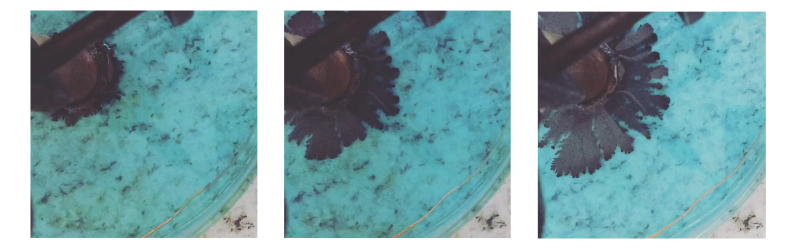
\includegraphics[width=14cm]{Figure6} \caption{Three subsequent frames of electrochemically deposited copper on a Petri dish in solution of $CuSO_4$ - experiment performed at Jagiellonian University, Institute of Physics}
\label{Fig6} 
\end{figure}

At the microscale  level several observations were made.
Studying the aggregation of silver nanoparticles, subject to an externally applied laser light, experimenters \cite{Ito:2013fh} measured a shift of the surface plasmon resonance spectrum towards the 1,064nm wavelength of the driving field.
In another study \cite{Carnall:2010ju}, mechanical work was used to agitate amyloid fibres and led to exponential growth of fibres of finite length. The physical mechanism leading to dissipation in this case, was the snapping of fibrils longer than optimal length for the given driving conditions.
The most intriguing, but yet open case of biological molecular machines, such as ATP- or GTPase, in multi-protein mixtures hold great promise for observation of dissipative adaptation. The conformational changes happen there, in discrete events of chemical dissipation through hydrolysis of triphosphates accompanied by interparticle interactions \cite{Schaller:2010cq}.

One can see that the presented possible realizations differ widely and it is probably fair to say, that the presented examples give more than preliminary support for the dissipative adaptation hypothesis for certain microscopic and also macroscopic many-body systems. 
For the establishment of a general principle of dissipation or growth of complexity more firm evidence will need to be gathered, together with a detailed analysis of the individual terms of equations (\ref{DissipationDrivenEq}) and (\ref{DissipationDrivenEq2}). All of this, of course, follows under the assumption of validity of the fluctuation theorems, therefore their further analysis is also desired.

%Finally, taking into account the information processing/storing capability of animate matter, one is led to a natural question - could there be a deeper relation behind the fluctuation theorem, perhaps involving information theory? Could fluctuation theorem be derived from it?

Nevertheless, those advancements push us towards understanding the origin of biological complexity and it is likely that the next steps, with the help of information theory, could help us understand the emergence of agency. 
In fact, purpose directed behaviour can be seen as a result of information processing and storage which itself relies on availability of free energy as shown by Landauer \cite{Landauer:2002wc}. Therefore, it is desired to somehow bridge the gap between physics and biology using a new principle, as proposed by Schrödinger (section \ref{SchrodingersInfluence}) - preferably including information theory. One of the paths one could choose for such an endeavour is the search of variational principles.

\section{Search for a unifying principle}
\label{UnifyingPrinciple}
The search for variational or extremization principles in physics has a long history of success. In classical mechanics, one finds the equations of motion from Lagrangian formalisms with the principle of least action. In thermodynamics and statistical physics of equilibrium state the principle of maximum entropy yields the true equilibrium states of a given system. 

In 1912, Ehrenfest was the first who asked whether such a principle for a yet unknown function could exist for non-equilibrium steady states \cite{Dewar:2014ek}.
The search, however, could be dated to the works of Kirchoff and Rayleigh and their least dissipation theorems, which development ceased immediately after the establishment of equilibrium statistical mechanics.
Interest in least dissipation principles was reborn in the 1950s due to joint paper of Onsager and Machlup \cite{Onsager:3UFhYpWV} which modeled small microscopic fluctuations (away from criticality) around exponential relaxation to equilibrium and which provided a "microscopic" basis for the least dissipation principle. The validity of the least dissipation principles, including Prigogine's MinEP, is however restricted to near-equilibrium states. In fact, in an example presented by Landauer \cite{Landauer:pJ4RYJRG}, the steady state was generating the maximum amount of entropy.

\subsection{MaxEP principle}
\label{MaxEPSection}
The example presented by Landauer, was however, not, the origin of the so-called maximum entropy production (MaxEP, sometimes called MEP) principle. The conjecture of MaxEP originated from some promising (but controversial) successes in studies of planetary climates \cite{Lorenz:J80tzZkl, Paltridge:2007jf, Kleidon:1339033} and since then was applied in a loose manner to other fields, such as fluid turbulence \cite{Ozawa:2003jt, MALKUS:2003ix} and crystal growth morphology \cite{Martyushev:2006ge}.
%In the case of Malkus's turbulence, it also allegedly hinted to some theoretical relationship between maximum irreversibility and dynamic stability, by the fact that MaxEP predicts the same dissipation functional as instability criterion in shear turbulence \cite{Dewar:2014ek}.

The main reasons that drove controversies, e.g. \cite{Goody:2007cv}, around those successes were the accuracy of the results and the \textit{ad hoc} and unsystematic manner in which MaxEP was applied.
For example, the earliest successes of MaxEP applied to Earth's climate were based on a 2-zone model where the energy balance and temperatures were obtained through maximization of entropy production (EP) associated with meridional heat transport in the atmosphere and the oceans, completely ignoring the dominant part of the total EP coming from radiative EP.

There are also different formulations of MaxEP \cite{Virgo:2010it, Zupanovic:2010ea, Kawazura:2010dy, Dewar:2005da}, many not really formalised, which were subjects to a pletora of readily available reviews, e.g. \cite{Bruers:2006us, Zupanovic:2010bv, Dewar:2014ek}. To author's best knowledge, all versions were predicting, a time independent probability distribution function, therefore, a detailed review of individual differences will not be undertaken in this work.
Instead, we will comment on the most common formulation from the point of view of dissipation function and then present what seems to be, the most promising idea.

The usual working formulation of MaxEP  principle states that \textit{for systems admitting a spectrum of possible steady states, MaxEP says that the system is most likely to be found in steady state  with the greatest entropy production}. Directly from this statement the relation between MaxEP and Prigogine's MinEP becomes clear.

\subsubsection{Relation to MinEP}

For linear, near-equilibrium systems that only admit a single steady state, MinEP states that system's steady state produces less entropy than any possible transient state.
MinEP compares steady states with transient states.

For some not yet determined class of nonlinear, far from equilibrium systems that admit multiple steady states, MaxEP states that the system settles in the steady state with the greatest entropy production. MaxEP compares steady states to other steady states, staying silent on transient states.

\subsubsection{Extrema of the Dissipation Function and MaxEP}
The dissipation function is similar to the entropy production, and although it is not directly connected to a state function, the various fluctuation theorems provide exact, non-equilibrium relations. Given this similarity, it is interesting to see how consistent with it might be the MaxEP principle. 

If we consider a special case of equation (\ref{distributionPropagator}) when the system is driven i.e. dissipation is given by equation (\ref{primaryDissipationFunction}), then we obtain:
\begin{equation}
  f(\bm{\Gamma};t)=f(\bm{\Gamma};0)\exp[-\beta \int_0^t ds\ V\bm{J}(\bm{\Gamma}_{-s})\cdot \bm{F}_e(t-s)]
\end{equation}
from which it is clear that the probability of observing the phase $\bm{\Gamma}$ at time $t$ is increased if the integrated dissipation terminating at phase $\bm{\Gamma}$ and time $t$ is large and positive. Furthermore, we suspect that the dissipation term will, at long times, dominate over the initial probability distribution, thus justifying MaxEP as a good approximation.

Moreover, considering equation (\ref{DissipationTheorem}) with $B=\Omega$, one can see, that if, the autocorrelation function $\langle \Omega(\bm{\Gamma})\Omega(\bm{\Gamma}_t)\rangle$ decays monotonically with time, then the value of the ensemble average of the instantaneous dissipation function, $\langle \Omega(t) \rangle$ will be have a higher value when it reaches its steady state than for any other state it passes through. The system should therefore expose itself to a steady state of maximium dissipation.
The assumption of monotonicity of the autocorrelation function of course doesn't hold in all cases. Through numerical simulations done in \cite{Brookes:2011hu} it was shown that the dissipation average sometimes peaks to a higher number before reaching a stable steady state value. 
One should note here, that in the light of formulation of MaxEP from section \ref{MaxEPSection}, this result doesn't prove or disprove the MaxEP principle as MaxEP compares steady states to steady states.
It's simply the instantaneous dissipation that is not necessarily maximized at all times.

%In order to provide further information on the behaviour of the dissipation function, one should consider a system where multiple steady state solutions are known to exist. One such model was investigated by Zhang \cite{Zhang:2001jc} who considered heat flow in a one-dimensional lattice. In such model, two possible steady states exist - a soliton or a diffusive heat flow - and depend on the initial conditions and the field strength.
%For a given field strength, there is a certain set of trajectories from which a soliton emerges spontaneously. There's also a critical value of the field strength after which the probability of forming a soliton is equal to unity. This chaos-soliton transition becomes sharper as the size of the system (number of particles) is increased. 
%One might think that it may very well be that after increased simulation time the transition becomes sharper as well, but it turns out, that even for zero-field there exists a set of initial conditions (of zero measure) that also form a soliton. This peculiar points of the phase space form a basin of attraction which grows after the external field is increased. This non-uniqueness of the steady state stands in contrast to other 1D and 2D numerical simulations like \cite{Maeda:1995bj}.

%Those examples might suggest that the strong conjecture of MaxEP might not hold for all steady state or that the field strength should also be considered a constrain of the system.
%Perhaps, MaxEP requires the external forcing to be sufficiently large that low entropy states are unstable. It is clear that the results will depend on the constraints imposed, and therefore the problem could be reformulated as a problem in identification of the appropriate constraints.

The (mostly) negative statements with regards to MaxEP, one finds in the works of Evans \cite{Evans:2241458}, seem to be referring to a universal MaxEP principle valid at all times, rather than to some approximation.
There are of course valid reasons for scepticism about MaxEP as a general law. In an extensive analysis analysis of family of dissipation functionals of the form $f= D(D_v/D_m)^n$ and $f= D_m(D_v/D_m)^n$ for $n\geq 0$, involving the total dissipation $D$, dissipation in the mean flow $D_m$, and dissipation in the fluctuating flow $D_v$, Kerswell \cite{Kerswell:2002bw} was unable to identify a universal dissipation functional that applied to all flow problems.
Finally, the study of generic MaxEP hypotheses through numerical simulations at the microscopic level is rather hard, because systems that generate multiple steady states, such as convection and turbulent flow, are computationally very expensive.
 
\subsubsection{MaxEnt based formulations of MaxEP}

Perhaps the most promising interpretation of MaxEP principle, put forward by Dewar\cite{Dewar:775452, Dewar:2009fg, Dewar:2005eo}, assumes that MaxEP is not a physical principle at all. Instead, by analogy to Jaynes MaxEnt it is an inference method i.e. a method for deducing the most unbiased predictions from an incomplete set of statistical data. In the light of this interpretation, problems with finding maximum entropy production in a given model, may be related to \textit{the way} the principle was applied, i.e. finding the right constraints and not to the principle itself.
Instances of apparent failure were noted in phenomenological models of heat flow in plasma/fluid system \cite{Kawazura:2010dy}, where maximum as well as minimum was observed depending on how the system was driven, and also in the climate general circulation models (GCM), where no extremum of EP was not found \cite{Dewar:2014ek}.
Whether those failures can indeed be justified by unlucky selection of constraints remains to be shown. Nevertheless, a precocious procedure was proposed by Dewar which involves three steps.

The first step is done by narrowing the scope of validity. We notice that systems that are weakly driven have (neglecting the set of measure zero) only one steady state available.\footnote{Of course, in principle, there is always only one stationary state when our knowledge about the system is full, however, by assumption, in case of strongly driven systems our ignorance is much greater and there is more room for an inference principle.} Therefore there is no room for MaxEP to operate and we instead focus on systems driven strongly in far for equilibrium regime.
Two classic examples of far from equilibrium systems involve \textit{shear turbulence} with Reynolds numbers greater than the critical value necessary for the onset of turbulence and \textit{Rayleigh-Bénard} cell with Rayleigh numbers greater than the critical value necessary for the onset of convection.
In those scenarios both examples exhibit many flow solutions allowed when we apply only a restricted set of stationary conditions rather than the full dynamics.
%TODO: Place for work of Ozawa

Secondly, Dewar introduces information theoretical measure of the distance from equilibrium, or \textit{irreversibility} $I$ (similar to the one defined in equation \ref{IrreversibilityMeasure}), defined in terms of the relative probabilities of forward and reverse fluxes. 
The first demand (dynamical instability) is then reformulated as a strong inequality constraint $I>I_{min}$. 
Then using procedures known from MaxEnt it is shown that $I$ adopts its maximum possible value under the stationarity constraints.

The final step consists of reinterpretation of $I$ as thermodynamic entropy production. In this derivation of MaxEP, entropy production depends on the applied constraints.

The just outlined procedure (which is Dewar's third iteration of the principle) is presented in the proceeding section in detail.

\subsection{MaxEP principle as an inference principle}
\label{MaxEPInferenceSection}
We will consider a general open system (volume $V$, boundary $\Omega$) which exchanges both matter and energy with its surroundings. The system may consist of several components.
The presence of fluxes, both within the system, and between the system and its environment is the primary characteristics of the non-equilibrium stationary states. We'll denote the instantaneous value of those fluxes, by the vector $\bm{f}$. The flux vector $\bm{f}$ may be related to some local density $\rho$ with the use of the continuity equation $\partial \rho / \partial t =  - \nabla \cdot \bm{f} + h$, where $h$ denotes a local source; alternatively (for example in case of Navier-Stokes equations), the components of $\bm{f}$ might themselves be identified with local densities. Macroscopic state of the system is then described by $\bm{f}$ (or $\rho$) with the stationarity condition given by equation (\ref{SteadyStates}).
Similarly to the MaxEnt we maximize the relative entropy
\begin{equation}
  H = - \int p(\bm{f})\ln \frac{p(\bm{f})}{q(\bm{f})} d\bm{f},
\end{equation}
with respect to probability distribution function $p(\bm{f})$, subject to given dynamical constraints $C$, where $q(\bm{f})$ is a prior probability distribution function, with the symmetry $q(\bm{f}) =q(\bm{-f})$ which corresponds to zero flux state $\bm{F}= \int q(\bm{f}) \bm{f} d\bm{f}=0 $.
By Gibbs' inequality, $H \leq 0$ with equality if and only if $p(\bm{f})=q(\bm{f})$.
The constraints represented by $C$ are written in the generic form of functionals of fluxes $\phi_m(\bm{f})$ and labeled by $m$:

\begin{equation}
\label{Constrain1MEP}
  \int p(\bm{f})\phi_m(\bm{f})d\bm{f} =0,
\end{equation}
which we can demand without loss of generality to be zero.
We also have the normalization constraint
\begin{equation}
\label{Constrain2MEP}
  \int p(\bm{f})d\bm{f} = 1.
\end{equation}
Now, in order to enforce the multiplicity of stationary states we introduce the \textit{irreversibility} defined by the Kullback-Leibler (KL) divergence of $p(\bm{f})$ and $p(-\bm{f})$:
\begin{equation}
\label{IrreversibilityMeasure}
  I= \int p(\bm{f}) \ln \frac{p(\bm{f})}{p(-\bm{f})} d\bm{f}.
\end{equation}
By Gibbs' inequality, $I \geq 0$ with equality if and only if $p(\bm{f})=p(-\bm{f})$, so that $I=0$ corresponds to the equilibrium state $\bm{F} = \bm{0} $.
Making the first step of the procedure, we demand that there is a state characterized by minimal irreversibility, $I>I_{min}(C)>0$, the value of which depends on the stationarity conditions $C$ of equation (\ref{Constrain1MEP}).
Those conditions should also determine the upper bound $I \leq I_{max}(C)$ by assumption.

Additionally we introduce a trial mean flux $\bm{F}$ (which is subsequently relaxed) via the auxiliary constraint
\begin{equation}
\label{Constrain3MEP}
  \int p(\bm{f})\bm{f} d\bm{f} = \bm{F}.
\end{equation}
The motivation for introducing $\bm{F}$ is to allow one to establish an extremal principle whereby $\bm{F}(C)$ is determined by varying the trial solution $\bm{F}$\footnote{This approach is analogous to the way in which equilibrium variational principles (e.g. minimum free energy) can be derived from MaxEnt by enlarging the set of fixed macroscopic variables $X$ to include one or more free unconstrained variables $Y$, then maximizing $S=H_{max}(X,Y)$ with respect to $Y$ with $X$ held fixed.}.
Under given constraints the MaxEnt solution for $p(\bm{f})$ is given by 
\begin{equation}
\label{MaxEntPDF1}
  p(\bm{f})^* = q( \bm{f} ) Z^{-1} \exp[\bm{\lambda} \cdot \bm{f}+ \bm{\alpha} \cdot \bm{\phi} (\bm{f}) - \mu ( d(\bm{f}) - e^{-d(\bm{f}))}],
\end{equation}
where $d(\bm{f})= \ln{p(\bm{f})/p(-\bm{f})}$, $\phi(\bm{f})$ denotes the vector with components $\phi_m(\bm{f})$, $Z = Z(\lambda, \bm{\alpha},\mu)$ is a normalisation factor (partition function) and $\bm{\lambda}$, $\bm{\alpha}$ and $\mu$ are Lagrange multipliers for (\ref{Constrain3MEP}), (\ref{Constrain1MEP}) and the upper-bound inequality $I<I_{max}$ respectively. The maximized relative entropy is given by:
\begin{equation}
  S(\bm{F}, I_0, C) \equiv H_{max} = \ln Z(\lambda, \bm{\alpha}, \mu) - \bm{\lambda} \cdot \bm{F} + \mu(I_0 -1).
\end{equation}

The next step involves maximizing $S(\bm{F}, I_0, C)$ with respect to the trial flux solution $\bf{F}$ with $I_0$ held fixed.
In the absence of the dynamic instability condition $I>I_{min}(C)$, MaxEnt predicts the basal state $I=I_{min}(C)$, i.e. minimal irreversibility, but when the basal state is excluded by the dynamical instability condition MaxEnt predicts a probability distribution function for which $I=I_{max}(C)$ i.e. maximal irreversibility which is characterized by $\mu =0$ and equation (\ref{MaxEntPDF1}) becomes:
\begin{equation}
\label{MaxEntPDF2}
  p(\bm{f})^* = q( \bm{f} ) Z^{-1} \exp[\bm{\lambda} \cdot \bm{f}+ \bm{\alpha} \cdot \bm{\phi} (\bm{f})].
\end{equation}
The intermediate solutions not predicted by this procedure would then correspond to transient states, between equilibrium state and the non-equilibrium stationary state.
The predicted irreversibility measure (equation \ref{IrreversibilityMeasure}) is then given by a functional of $\bf{F}$:
\begin{equation}
  I(\bm{F}) =2\ \lambda(\bm{F}) \bm{F} + 2\ \bm{\alpha(\bm{F})} \Phi^A(\bm{F}),
\end{equation}
where 
\begin{equation}
  \Phi^A(\bm{F}) \equiv \frac{1}{2} \int p(\bm{f})[\bm{\phi}(\bm{f})-\bm{\phi}(\bm{-f})]d\bm{f},
\end{equation}
is the expectation value of the anti-symmetric part of $\bm{\phi}(\bm{f})$. One may now notice that if the vector $\bm{\phi}$ is anti-symmetric or symmetric then (after adding the condition given by equation (\ref{Constrain1MEP})) the $\bm{\Phi}^A =0$, and the irreversibility measure reduces to:
\begin{equation}
\label{SymmetricIrreversible}
  I(\bm{F})=2 \bm{\lambda}(\bm{F})\bm{F}.
\end{equation}
%On the other hand when $\bm{\Phi}^A$ displays no pure symmetry then
%\begin{equation}
%\label{NonSymmetricIrreversible}
%  I(\bm{F}) = 2\ \bm{\alpha(\bm{F})} \Phi^A(\bm{F}).
%\end{equation}
A result consistent with the conclusion that there are no general expressions for thermodynamic entropy independent of the constraints.

\subsubsection{Relation to fluctuation theorem and dissipative adaptation}
In his first approaches, Dewar claimed to derive \cite{Dewar:775452, Dewar:2005eo} the fluctuation theorem from MaxEP. The claims in the more recent works are more modest \cite{Dewar:2014ek}. MaxEP there (and here) described, is in fact an approximation to the fluctuation theorem. Conclusion immediately obvious, regarding the fact that the fluctuation theorem also describes the non-steady states.
The irreversibility measure $I$ defined for MaxEP is related to the dissipation function $\Omega_t$ of equation (\ref{Dissipation}) through $I=\langle \Omega_t \rangle$, if we interpret the flux vector $\bm{f}$ as a time-average over time $t$. 

Furthermore, in the light of our discussion on dissipative adaptation given in section \ref{DissipationAdaptationSection}, it seems likely that MaxEP could give a reasonable approximation of a driven steady state in the long time limit. The usefulness of its predictions, would however, be dependent on the range of applicability of dissipative adaptation hypothesis, which is currently under investigations.
In any case, contrary to our expectations from the ending of the section \ref{DissipationAdaptationSection}; the presented variational approach is not more fundamental and at most helps in understanding the more likely final states, rather than their emergence. Complexity \textit{growth} is therefore better addressed by the dissipative adaptation hypothesis than MaxEP.
However, in order not to belittle the result of MaxEP, which practical implications could still be of great use, we would like to see how it applies to the phenomena of planetary climates.

\subsubsection{Example application for planetary atmospheres}

In this section we will describe an example application of MaxEP to planetary climates, therefore justifying ad-hoc hypotheses made in \cite{Paltridge:2007jf}\cite{Lorenz:J80tzZkl}.
The constraints in this model 1D box model are given by a simple radiative balance between total incoming short-wave (SW) irradiance and the total outgoing long-wave (LW) irradiance:
\begin{equation}
\label{BalanceEq}
  \sum_i F_{SW,i}= \sum_i F_{LW,i},
\end{equation}
where the sum goes over all latitudinal zones. The meridional heat fluxes are identified as $\bm{f}=\{f_i\}$ where $f_i$ is the flux from zone $i-1$ to zone $i$. 
The local (for each zone) equation has then the form
\begin{equation}
  F_{SW,i}- F_{LW,i} + \Delta F_i = 0.
\end{equation}
where $\Delta F_i = F_i - F_{i+1}$ and $\int p(\bm{f})\bm{f} d\bm{f}=\bm{F}=\{F_i\}$. 
The basal equilibrium state corresponds then to radiative equilibrium $F_{SW,i}= F_{LW,i}$ with $\bm{F}=\bm{0}$ and $I=I_{min}$. Having understood the constraints we can now rewrite the equation (\ref{BalanceEq}) as a condition
\begin{equation}
  \int p(\bm{f})\phi_1(\bm{f})d\bm{f} =0,
\end{equation}
with antisymmetric functional $\phi_1(\bm{f})=\sum_i \Delta f_i$. 
One can show that the Lagrange multiplier $\lambda = - \Delta (\frac{1}{T_i}) = \frac{1}{T_{i+1}}-\frac{1}{T_i}$ by considering a slight modification (non-steady state) of equation (\ref{MaxEntPDF2}) in which in zone $i$ energy $u(\tau)$ is stored for some finite time $\tau$ \cite{Dewar:2014ek}. 
Using the equation (\ref{SymmetricIrreversible}) we get our final result:
\begin{equation}
\begin{aligned}
  I(\bm{F})=2 \bm{\lambda}(\bm{F})\bm{F} \propto - \sum_i F_i \Delta\bigg(\frac{1}{T_i}\bigg)= \sum_i \bigg(\frac{\Delta F_i}{T_i}\bigg),
\end{aligned}
\end{equation}
which has the form of entropy production function used by \cite{Paltridge:2007jf, Lorenz:J80tzZkl}.
Further examples can be found in \cite{Dewar:2014ek}.
\section{Summary}

After over 100 years, the arguments of Boltzmann and others on the Loschmidt paradox have become more tangible and very refined. In this work we have shown how a quantitive description can be obtained from simple rules of Bayesian inference and post-diction, attributing irreversibility to our ignorance, limited predictive abilities and causality.
The obtained measure of irrevesibility is also a new example of fluctuation theorem, studies of which will follow in authors subsequent works.

The research on fluctuation theorems in gerenal has been immensely productive, providing us with better understanding of thermostated systems, steady states, dissipation and relaxation processes, while keeping the correspondence with linear response theory. Nevertheless, the limits of its generality are still being researched, while the applications of fluctuation theorem are already giving us new methods of calculating free energy of large molecules and some early understanding of self-replicators, dissipation driven self-assembly and the origin of complexity growth. As a final reflection on dissipative adaptation as the possible mechanism of complexity growth, we remark that it is consistent with the empirical observations of Eric Chaisson \cite{Chaisson:QaChIy8J, Chaisson:inPaa3oF} on free energy rate density measure of complexity.

Furthermore, in the present work we conclude, that the principle of MaxEP, as formulated by Roderick Dewar, stays in agreement with, the more general, fluctuation theorem and can be seen as a final state of dissipative adaptation. An independent (from dissipative adaptation) proof of its validity, remains an elusive task given its non-physical nature and arbitrariness in finding the appropriate constraints. An interesting future perspective would be compare this line of work with the concept of maximum entropy random walks.

The author hopes to continue his research in the field of non-equilibrium statistical mechanics, acknowledging that the full understanding of agency, life-like forms and complexity growth in general, will almost surely, demand a subtle inclusion of information theory and perhaps, a shift to the quantum description \cite{Kurchan:2000uh}.


\newpage

\addcontentsline{toc}{section}{References}
\bibliographystyle{ieeetr}
\bibliography{Refs}


\end{document}